\documentclass[12pt,a4paper]{article}

% Essential packages
\usepackage[utf8]{inputenc}
\usepackage[margin=2.5cm]{geometry}
\usepackage{graphicx}
\usepackage{float}
\usepackage[hidelinks]{hyperref}
\usepackage{booktabs}
\usepackage{pgfplots}
\usepackage{appendix}

% Document title and author information
\title{\textbf{Enhancing DAEN Program Effectiveness: Analysis of Alumni Interview Feedback at George Mason University}}
\author{James Baldo, Lingyun Dai}
\date{\today}

\begin{document}

\maketitle

% Abstract
\begin{abstract}
This study examines the effectiveness of the DAEN program at George Mason University's College of Computing and Engineering through the first systematic analysis of alumni feedback. The research addresses a critical need to understand program outcomes and identify areas for curriculum enhancement based on industry demands. Through structured interviews with fourteen program alumni who graduated between 2019 and 2023, the study collected comprehensive data on employment trajectories, technical skill utilization, and program effectiveness.
The research methodology combined qualitative interview analysis with advanced data processing techniques, utilizing AWS services and natural language processing to generate standardized datasets for analysis. The findings provide valuable insights into employment outcomes, technology adoption patterns, and curriculum effectiveness that will inform strategic program improvements. This pioneering effort establishes a foundation for ongoing program assessment and offers actionable recommendations for curriculum development and alumni engagement strategies.

\vspace{12pt}
\textbf{Keywords:} DAEN, Alumni, Employment, Program, Data, Analysis, Skill, Interview, Industry
\end{abstract}

\newpage
\tableofcontents
\newpage

\section*{List of Abbreviations}
\begin{tabular}{ll}
DAEN & Data Analytics Engineering\\
AWS & Amazon Web Services\\
M.S. & Master of Science\\
NLP & Natural Language Processing\\
MS & Microsoft\\
ML & Machine Learning\\
\end{tabular}
\newpage

% 1. Introduction Section
\section{Introduction}
\subsection{Purpose}
The primary objective of this research is to evaluate the DAEN 
program's effectiveness through comprehensive alumni interviews. Through structured feedback 
obtained from program alumni, this study conducts a 
detailed analysis of employment outcomes and program performance 
metrics. These insights are instrumental in enabling the DAEN 
department to implement strategic enhancements to the program's curriculum development and technology integration.

\subsection{Readership}
The report is intended for the DAEN program academic and 
administrative personnel including leaderships, stackholders, 
and development team. The findings presented in this report will provide valuable insights for improving program effectiveness, curriculum design, and student outcomes.

\subsection{Document Structure}
This report is organized into seven main sections. The Introduction 
establishes the research context and objectives. The Problem 
Statement formulates the research questions and scope. 
The Data section outlines the interview-based data collection 
methodology, data processing methodology, data quality interpretation, and interview question design. The Analysis section details the data 
processing pipeline and techniques employed. The Visualization section presents the derived data visualizations 
and their interpretations. The Findings section synthesizes key 
insights obtained through visualizations. Finally, the Next 
Steps and Lessons Learned section proposes future research 
directions and methodological improvements.

\newpage

% 2. Problem Statement Section
\section{Problem Statement}
\subsection{Problem}
The DAEN program faces significant challenges in evaluating program effectiveness as this represents the first systematic effort to gather alumni feedback. The absence of a centralized alumni database and limited alumni engagement mechanisms create substantial obstacles in reaching program graduates. The research revealed several critical issues:
\begin{itemize}
\item Limited Cloud Technology Exposure: While most alumni work extensively with cloud platforms in their current roles, many received insufficient exposure to these technologies during their coursework.
\item Theoretical vs. Practical Balance: Alumni consistently highlighted a need for more hands-on projects, indicating a gap between theoretical knowledge and practical application.
\item Emerging Technology Integration: The curriculum requires updates to incorporate emerging industry trends such as AI Ethics, DataOps, and Machine Learning Operations.
\item Alumni Engagement: Establishing and maintaining contact with program graduates poses a significant challenge, impacting the program's ability to gather comprehensive feedback.
\end{itemize}


\subsection{Scope}
This 15-week research project encompassed the development of interview methodology, conduct of alumni interviews, and comprehensive data analysis. The project faced significant initial challenges in establishing contact with alumni, as no centralized database existed. Over 50 alumni were contacted through LinkedIn, resulting in 14 successful interviews. The scope included:
\begin{itemize}
\item Development of structured interview questions
\item Implementation of data collection protocols
\item Creation of data processing pipeline
\item Analysis and visualization of collected data
\item Compilation of program improvement recommendations
\end{itemize}
A valuable outcome of this research is the creation of an initial alumni contact database, which will be shared with the GMU alumni office to facilitate future engagement efforts.

\newpage

% 3. Data Section
\section{Data}
\subsection{Data Product - Questions}
The research design centered on a carefully structured set of interview questions designed to capture comprehensive insights about alumni experiences and outcomes. The questions were developed to gather both quantitative and qualitative data across several key domains:
\begin{itemize}
\item Academic Profile Assessment (Questions 1-2)
\item Career Progression Tracking (Questions 3-6)
\item Technical Skill Utilization (Questions 4, 7)
\item Program Value Assessment (Questions 8-10)
\item Post-Graduation Development (Question 11)
\end{itemize}
The interview questions were structured as follows:

\begin{itemize}
\item \textbf{Graduation Timeline}: "What year and semester did you graduate from the DAEN program?"

Purpose: Establishes temporal context for program experience. Enables trend analysis across different graduation cohorts.

\item \textbf{Degree Classification}: "Did you receive an M.S. or Certificate?"

Purpose: Identifies academic credential level. Allows for segmentation of outcomes by program type.

\item \textbf{Initial Employment}: "What was the title of your first job, the name of the company, and the general responsibilities?"

Purpose: Maps initial career placement outcomes. Enables analysis of program-to-career transition. Provides insights into entry-level positions for DAEN graduates. Helps identify common career entry points.


\item \textbf{Initial Technical Requirements}: "What technologies and tools did you use for this job title?"

Purpose: Documents technology requirements for entry-level positions. Helps align curriculum with industry entry requirements. Identifies potential gaps in technical preparation. Provides baseline for technology evolution tracking.


\item \textbf{Career Progression}: "What is your current job title, the name of the company and the general responsibilities?"

Purpose: Tracks career advancement patterns. Enables comparison between entry and current positions. Identifies common career progression paths. Helps understand long-term career outcomes.


\item \textbf{Job Mobility}: "How many jobs have you had since you graduated?"

Purpose: Measures career mobility patterns. Indicates job market dynamics for DAEN graduates. Helps understand typical career progression timelines.

\item \textbf{Technology Stack}: "List the most used technologies/tools in your career. (E.g. Programming language, framework, cloud, ML)"

Purpose: Identifies critical technical skills for career success. Maps evolution of technology requirements over time. Helps prioritize curriculum updates. Provides insights into industry technology trends.


\item \textbf{Program Value Assessment}: "What knowledge and skills that you acquired in the DAEN program have been the most valuable to your career? Can you specify the concepts/methodologies/technologies that were most valuable?"

Purpose: Evaluates curriculum effectiveness. Identifies most impactful program elements. Helps validate current course offerings. Guides future curriculum development.


\item \textbf{Gap Analysis}: "If DAEN program provided these specific courses, topics, or training, I would have been more prepared in my career..."

Purpose: Identifies curriculum gaps. Captures emerging industry needs. Guides program enhancement efforts. Provides direct feedback for improvement.


\item \textbf{Program Effectiveness}: "How well did the DAEN courses prepare you for your career? (Scale: 1 -- Not well at all, 5 -- Very good)"

Purpose: Quantifies overall program effectiveness. Provides comparative metric across graduation years. Enables objective program assessment. Facilitates trend analysis over time.


\item \textbf{Continuous Learning}: "Have you completed any courses/certifications since you graduated from the DAEN program?"

Purpose: Identifies post-graduation learning needs. Reveals industry certification preferences. Helps understand skill gap mitigation strategies. Guides potential certification partnership opportunities.
\end{itemize}

\subsection{Collection Process}
The data collection process followed a systematic approach designed to ensure consistency and quality:
\begin{itemize}
\item \textbf{Alumni Identification}
\begin{itemize}
\item LinkedIn network search using DAEN program keywords
\item Referral requests from identified alumni
\item Collaboration with faculty for alumni contacts
\end{itemize}
\item \textbf{Interview Platforms}
\begin{itemize}
\item MS Teams (primary platform)
\item Zoom (secondary platform)
\item LinkedIn messaging (alternative option)
\end{itemize}

\item \textbf{Recording Methods}
\begin{itemize}
\item Audio recordings (Teams and Zoom)
\item Automated transcription (Teams)
\item Direct text responses (LinkedIn)
\end{itemize}

\item \textbf{Data Security}
\begin{itemize}
\item Secure storage of recordings
\item Confidential handling of personal information
\item Anonymous processing of responses
\end{itemize}
\end{itemize}
\subsection{Data Process}
The data processing pipeline consisted of several structured stages:
\begin{itemize}
\item \textbf{Storage and Security}
\begin{itemize}
\item Upload to AWS S3 bucket
\item Encryption of sensitive data
\item Access control implementation
\end{itemize}
\item \textbf{Transcription}
\begin{itemize}
\item AWS Transcribe processing
\item Manual verification of transcripts
\item Format standardization
\end{itemize}

\item \textbf{Data Extraction}
\begin{itemize}
\item NLP toolkit implementation
\item Text tokenization and pattern matching
\item Keyword extraction and categorization
\end{itemize}

\item \textbf{Structure and Format}
\begin{itemize}
\item CSV file creation with 15 primary columns
\item Data transformation for visualization
\item Quality control checks
\end{itemize}
\end{itemize}

\subsection{Data Quality}
Interview-based research inherently presents various potential biases and data quality challenges that must be carefully considered and addressed. Drawing from established research methodology literature (Bergelson et al., 2022; Nikiforova, 2020) and implementing practical measures in our research process, we established the following quality control framework:
\begin{itemize}
\item \textbf{Interview Structure Implementation}
\begin{itemize}
\item Utilized a standardized set of 11 structured questions asked in the same order for all participants
\item Questions were designed to be neutral and open-ended to avoid leading the respondents
\item Interviewers maintained consistent protocols by not prompting or suggesting answers
\item Each interview followed the same format regardless of platform (MS Teams, Zoom, or written surveys)
\item Responses were accepted as given without attempting to influence or modify them
\end{itemize}
\item \textbf{Data Collection Quality Controls}
\begin{itemize}
\item Recorded all interviews (audio or text) with participant permission
\item Used AWS Transcribe consistently across all audio recordings to ensure uniform transcription quality
\item Applied the same NLP toolkit for all text extraction to maintain processing consistency
\item Implemented systematic data extraction procedures using local natural language processing tools
\item Maintained standardized formats for data storage and processing
\end{itemize}

\item \textbf{Data Processing Standards}
\begin{itemize}
\item Created a uniform CSV structure with 15 standardized columns for all interview data
\item Applied consistent text preprocessing tasks across all responses
\item Used automated Python scripts in AWS SageMaker for standardizing string formats
\item Implemented systematic handling of multiple responses through column expansion
\item Maintained data anonymity through consistent identifier formatting (CEC-DAEN-[Graduation Year]-[MS/Cert]-[Sequence Number])
\end{itemize}

\item \textbf{Quality Verification Procedures}
\begin{itemize}
\item Conducted human review of ambiguous responses
\item Filtered out unclear or inconsistent terminology
\item Applied standardized categorization for job titles based on industry classifications
\item Mapped similar technologies to standardized categories through comprehensive research
\item Verified data transformations through multiple review cycles
\end{itemize}
\end{itemize}
To ensure consistency and minimize bias in our data collection and processing:
\begin{itemize}
\item Interviewers proceeded systematically through questions without deviation
\item No additional prompting or clarifying questions were used that might influence responses
\item Raw responses were preserved in their original form before any processing
\item All data processing steps were documented and applied uniformly
\item Standardization procedures were based on established industry classifications rather than subjective interpretations
\end{itemize}
This systematic approach to data quality management was implemented to ensure that our findings would accurately represent the alumni feedback while minimizing potential biases or inconsistencies in data collection and processing.

\newpage

% 4. Analysis Section
\section{Analysis}
The analysis followed a structured approach to process and interpret the collected interview data:

\noindent\textbf{Step 1: Data Organization}
\begin{itemize}
\item Compilation of raw interview transcripts
\item Creation of standardized data templates
\item Initial categorization of responses
\end{itemize}
\textbf{Step 2: Data Processing}
\begin{itemize}
\item Text analysis using NLP techniques
\item Standardization of job titles and technologies
\item Category development for skills and tools
\end{itemize}
\textbf{Step 3: Visualization Development}
\begin{itemize}
\item Selection of appropriate visualization types
\item Implementation in Tableau
\item Iterative refinement based on patterns
\end{itemize}
\textbf{Step 4: Pattern Analysis}
\begin{itemize}
\item Identification of trends across graduation years
\item Analysis of technology usage patterns
\item Assessment of program satisfaction metrics
\end{itemize}

\newpage

% 5. Visualization Section
\section{Visualization}
% Include your graphs, charts, and visual representations
\begin{figure}[H]
    \centering
    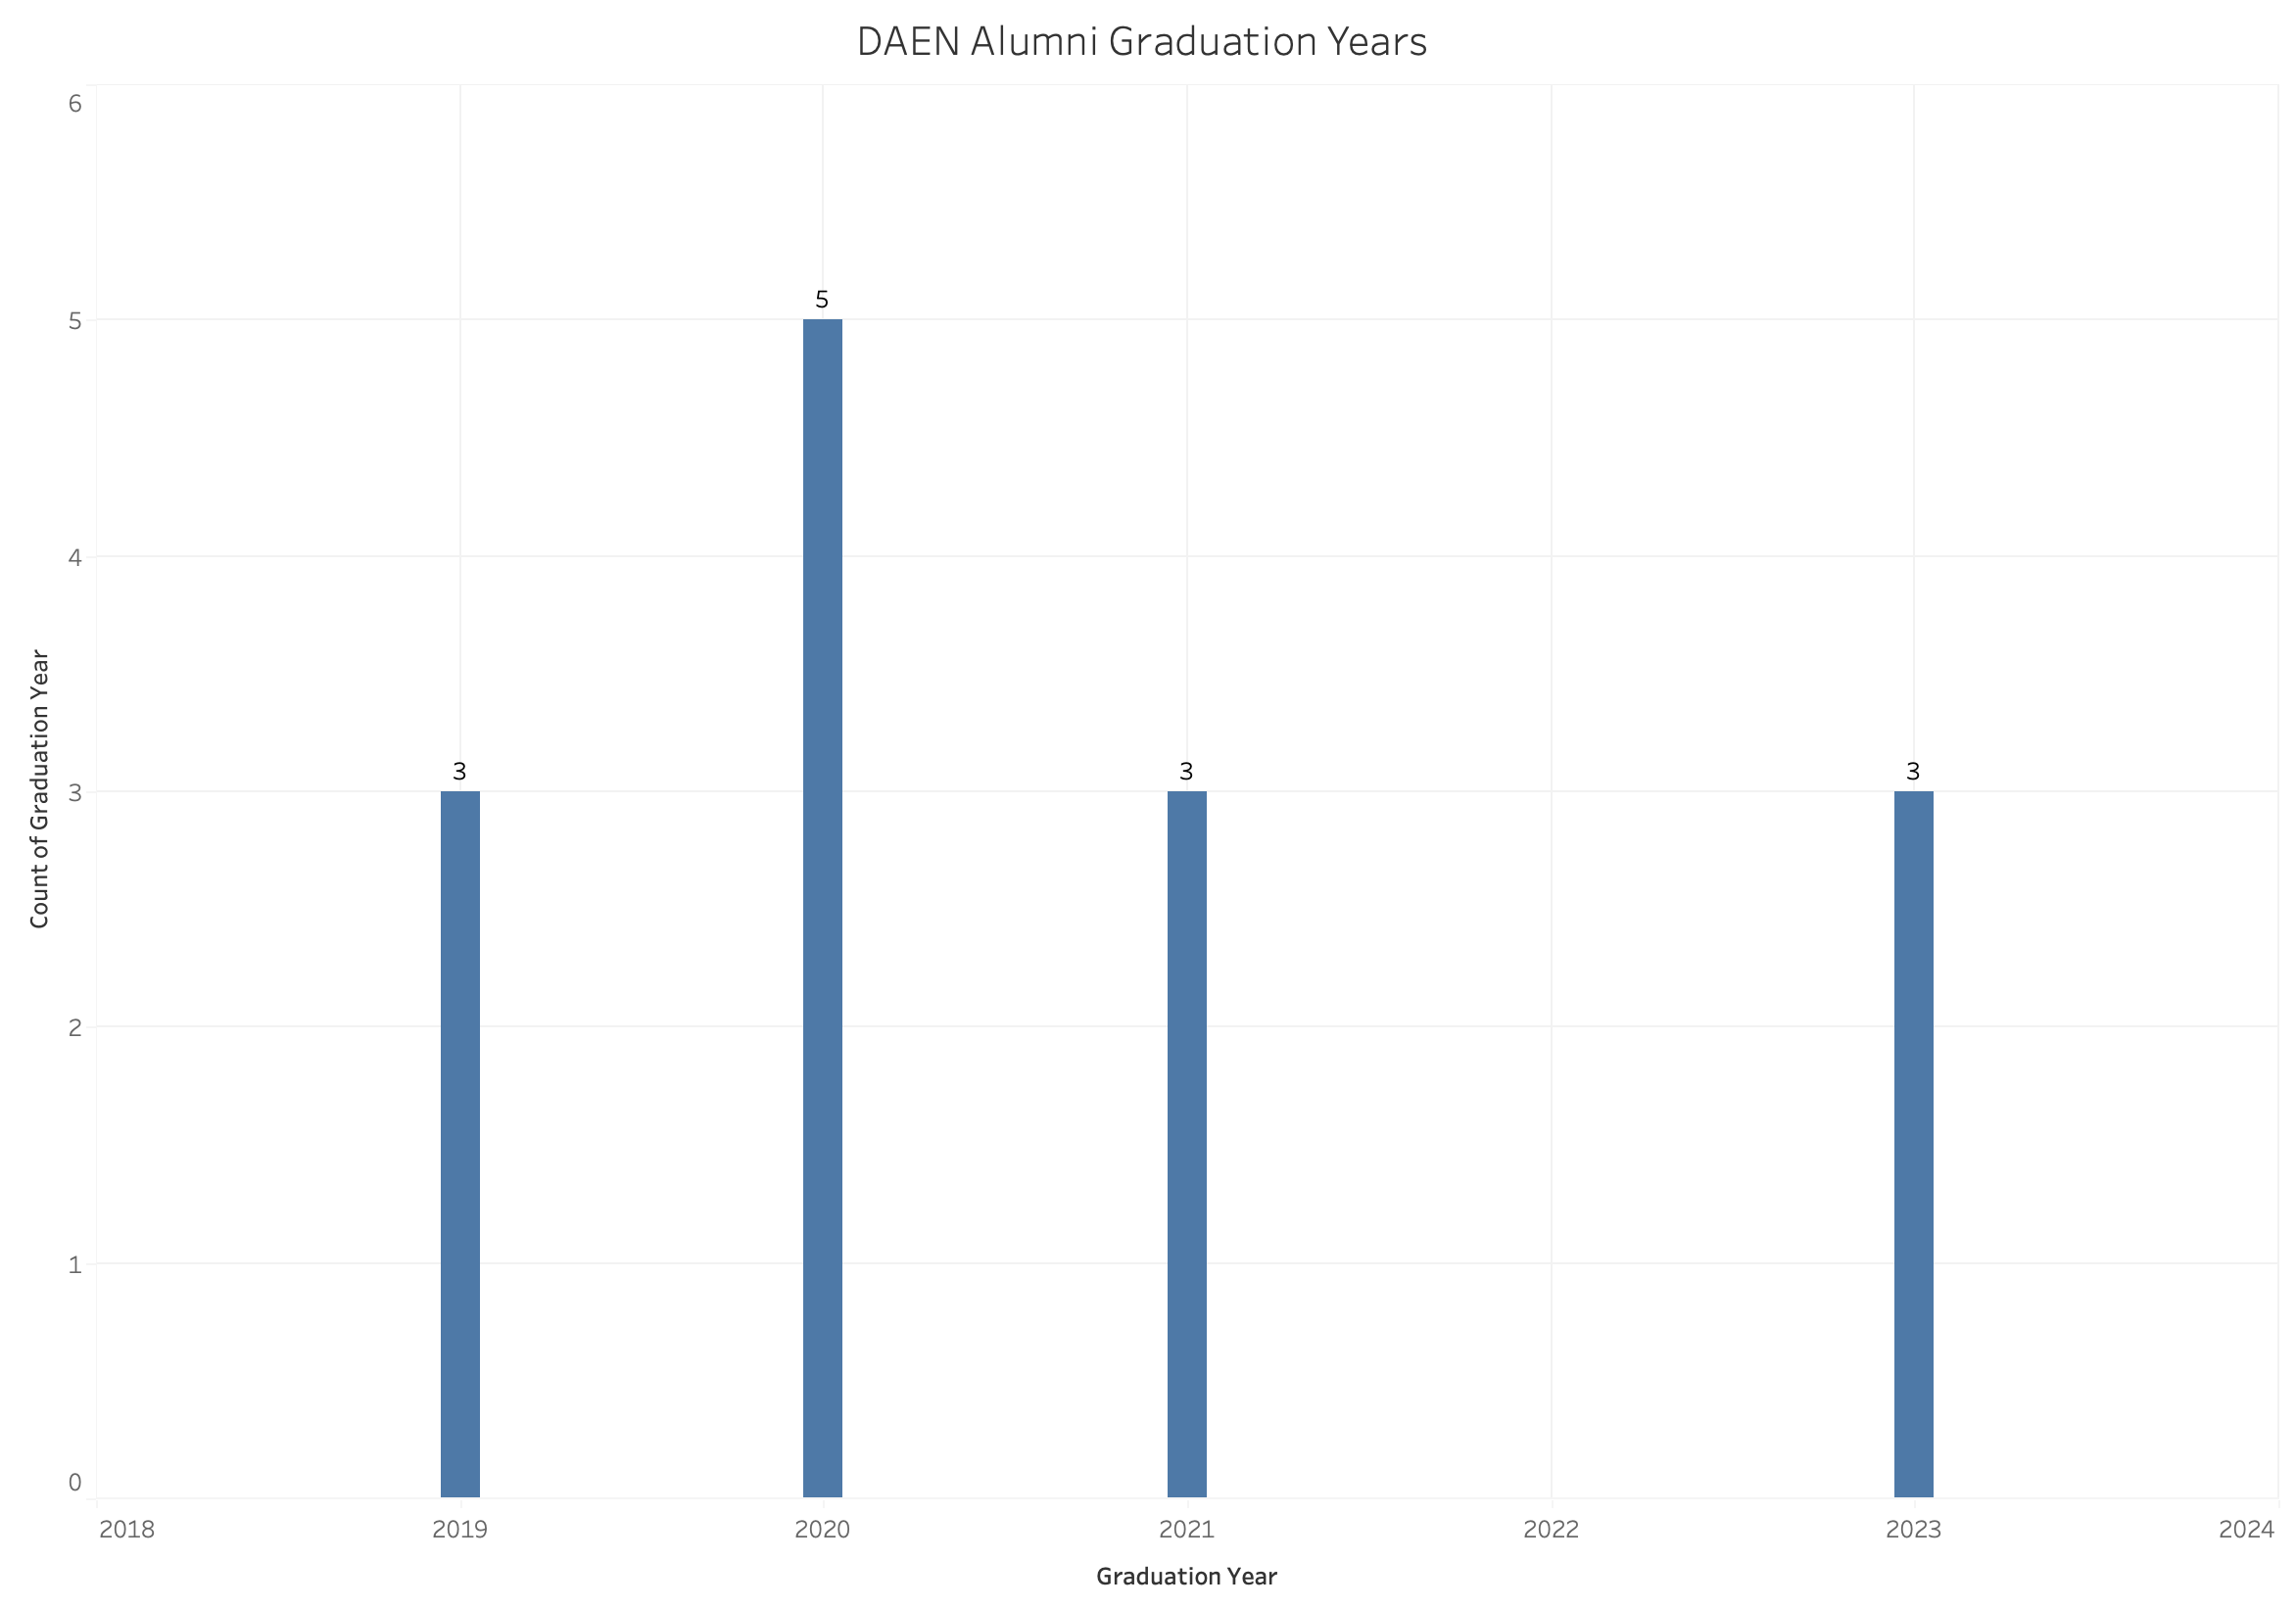
\includegraphics[width=0.9\textwidth]{visualizations/graduation-year.png}
    \caption{DAEN Alumni Graduation Year Distribution}
    \label{fig:graudation-year}
\end{figure}
The graduation year distribution reveals a concentration of respondents between 2019-2023, with the peak in 2020 (5 alumni). Notable challenges were encountered in reaching alumni who graduated before 2018.

\begin{figure}[H]
    \centering
    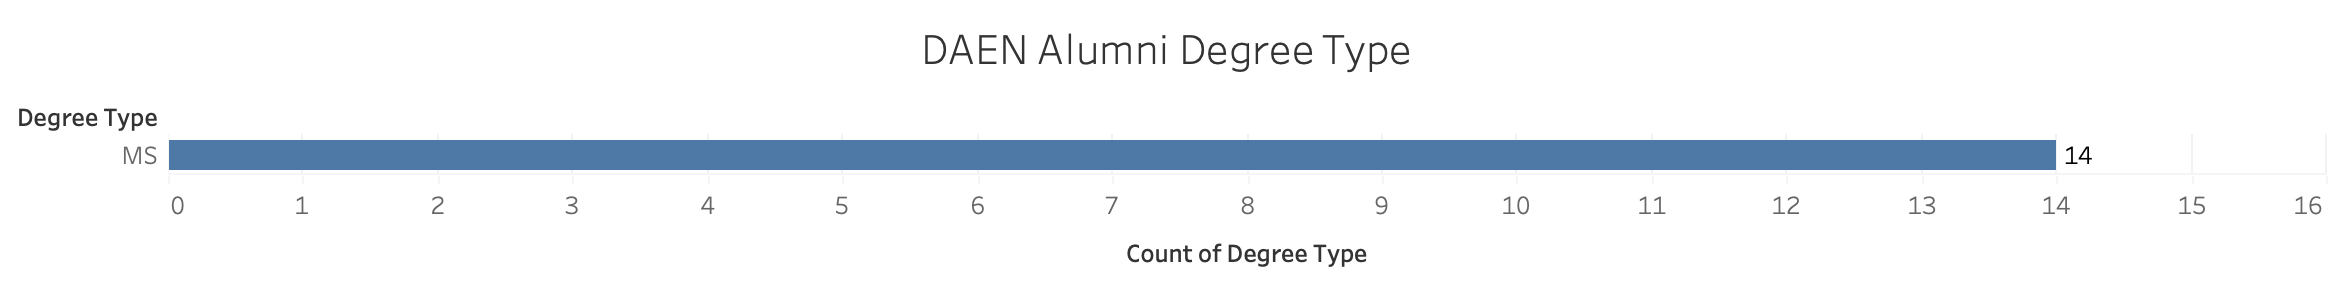
\includegraphics[width=0.9\textwidth]{visualizations/degree-type.png}
    \caption{DAEN Alumni Degree Type Distribution}
    \label{fig:degree-type}
\end{figure}
All respondents held MS degrees, indicating our sample represents the full-degree program experience. The absence of certificate holders suggests a need for targeted outreach to this alumni group.

\begin{figure}[H]
    \centering
    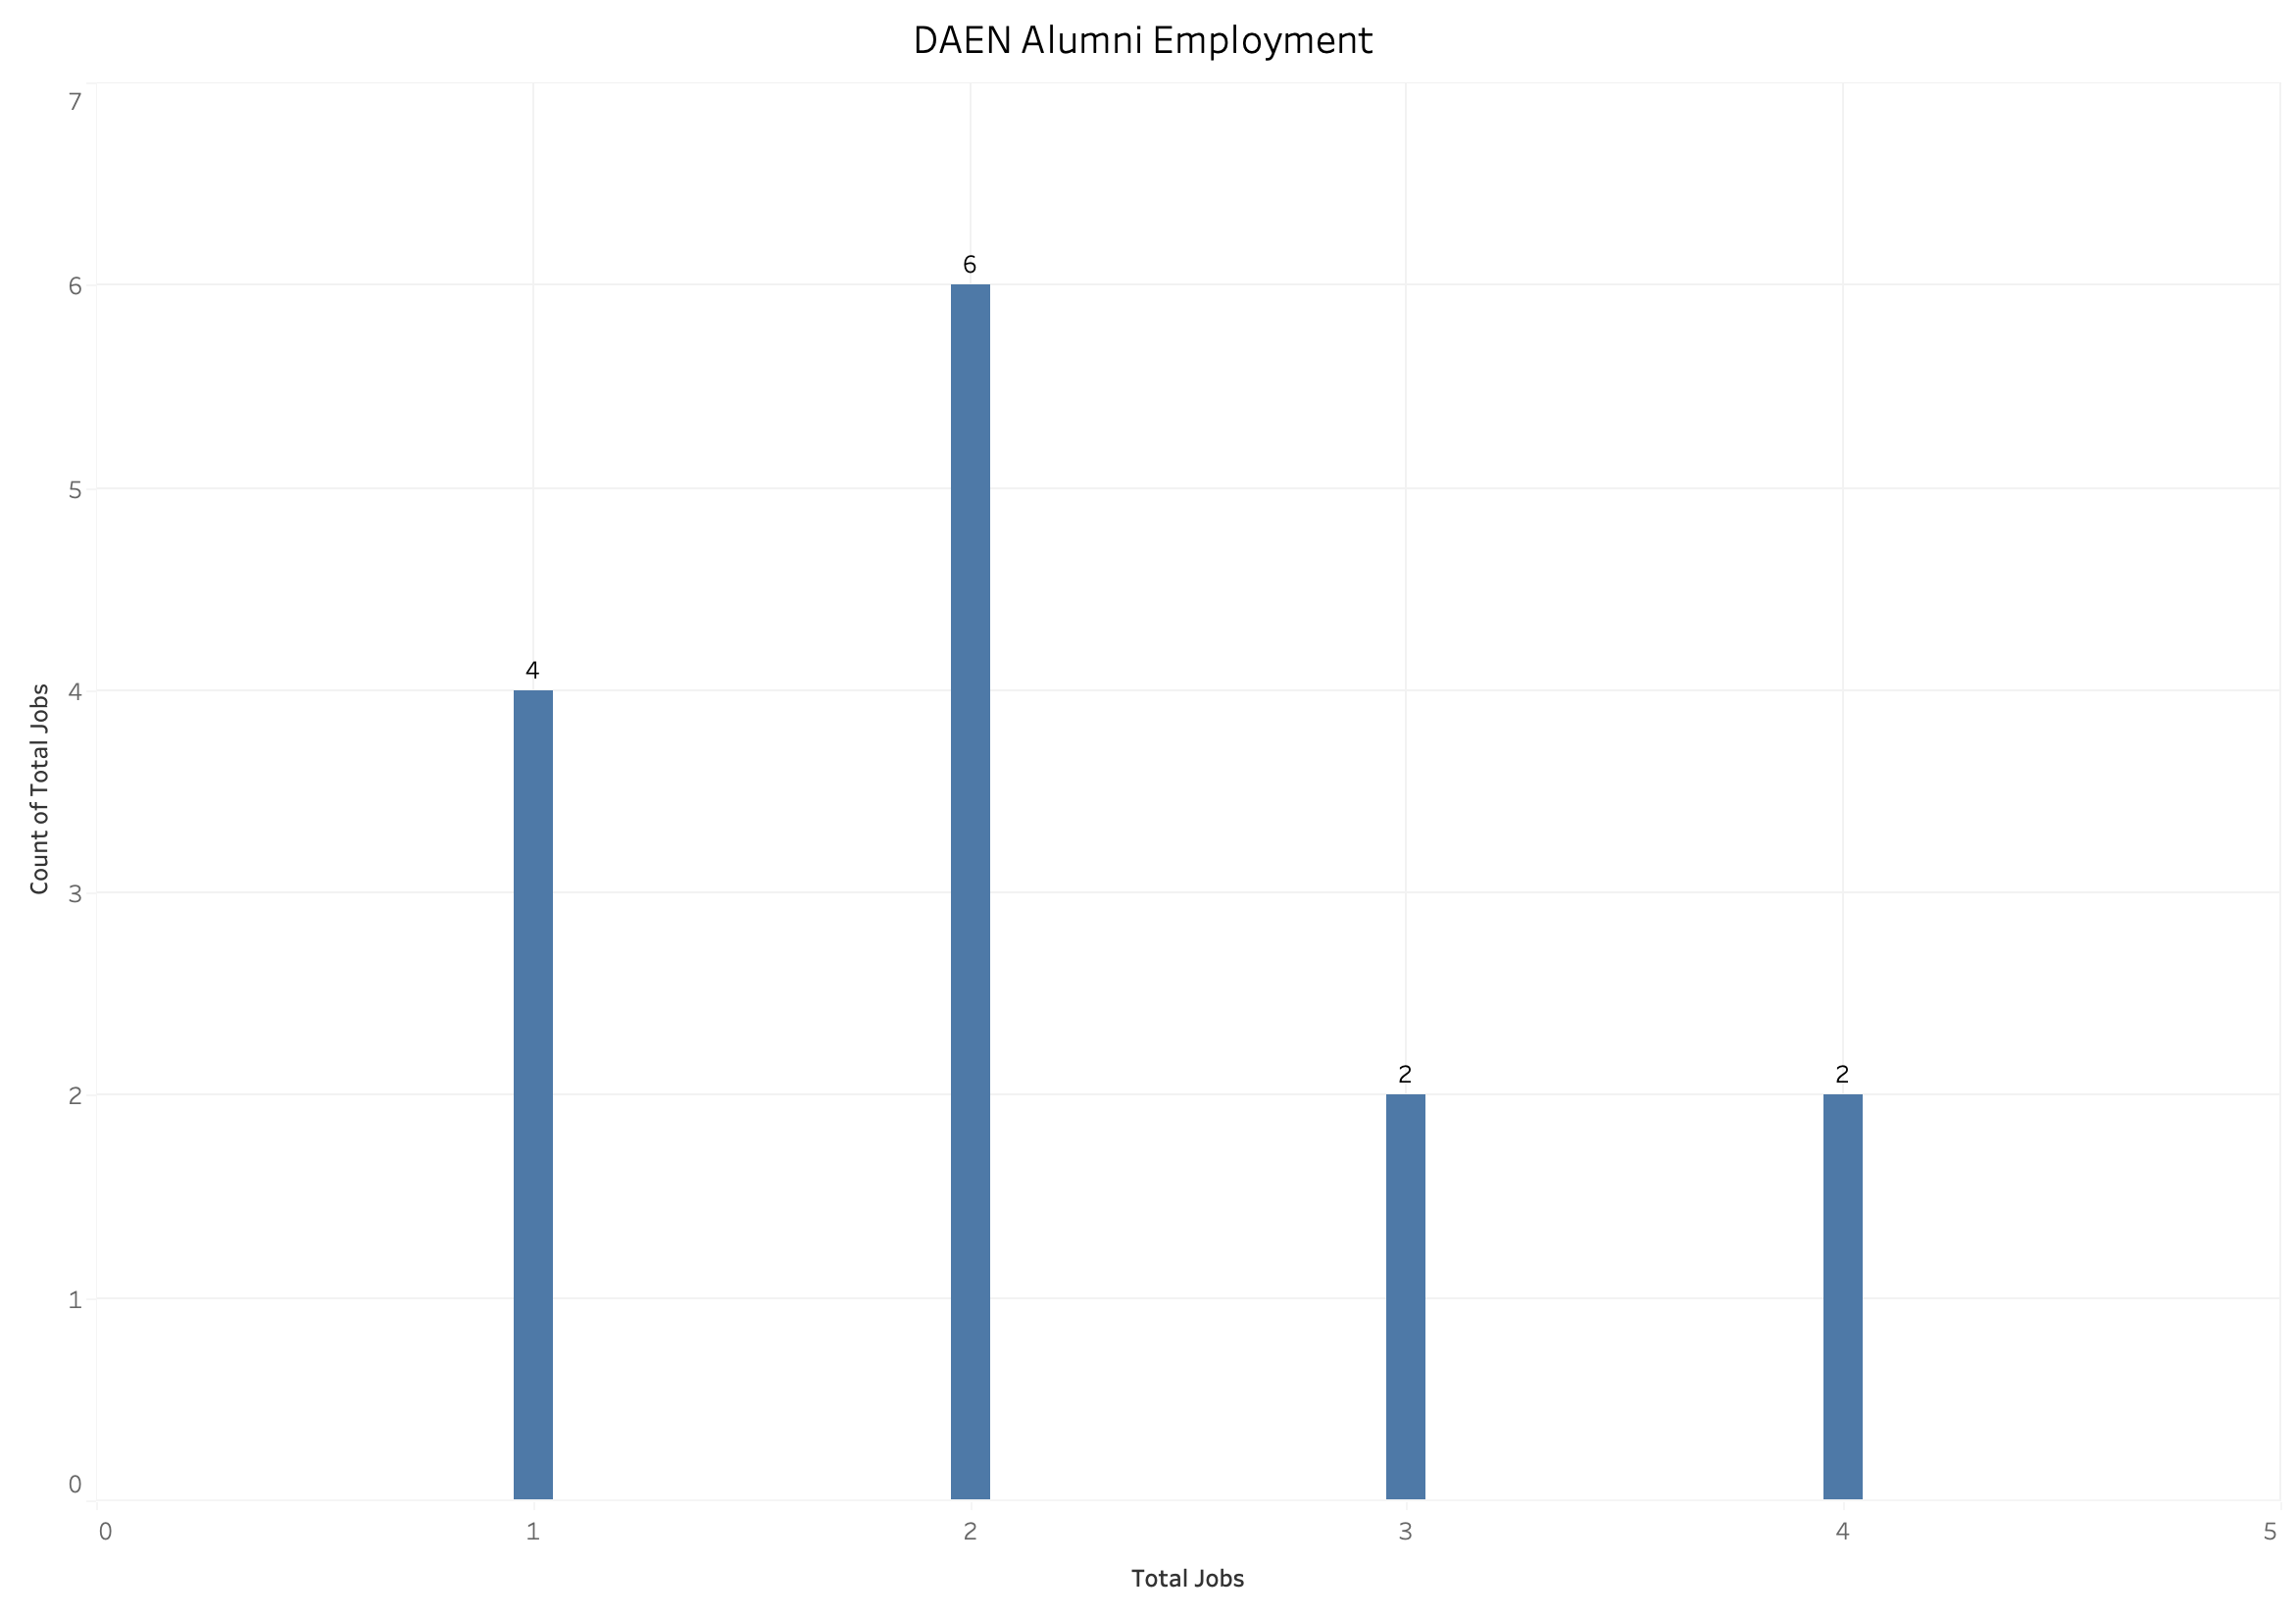
\includegraphics[width=0.9\textwidth]{visualizations/total-jobs.png}
    \caption{Total Jobs Held by DAEN Alumni}
    \label{fig:total-jobs}
\end{figure}
The analysis reveals that approximately 43\% of alumni have held two jobs since graduation, suggesting active career progression.

\begin{figure}[H]
    \centering
    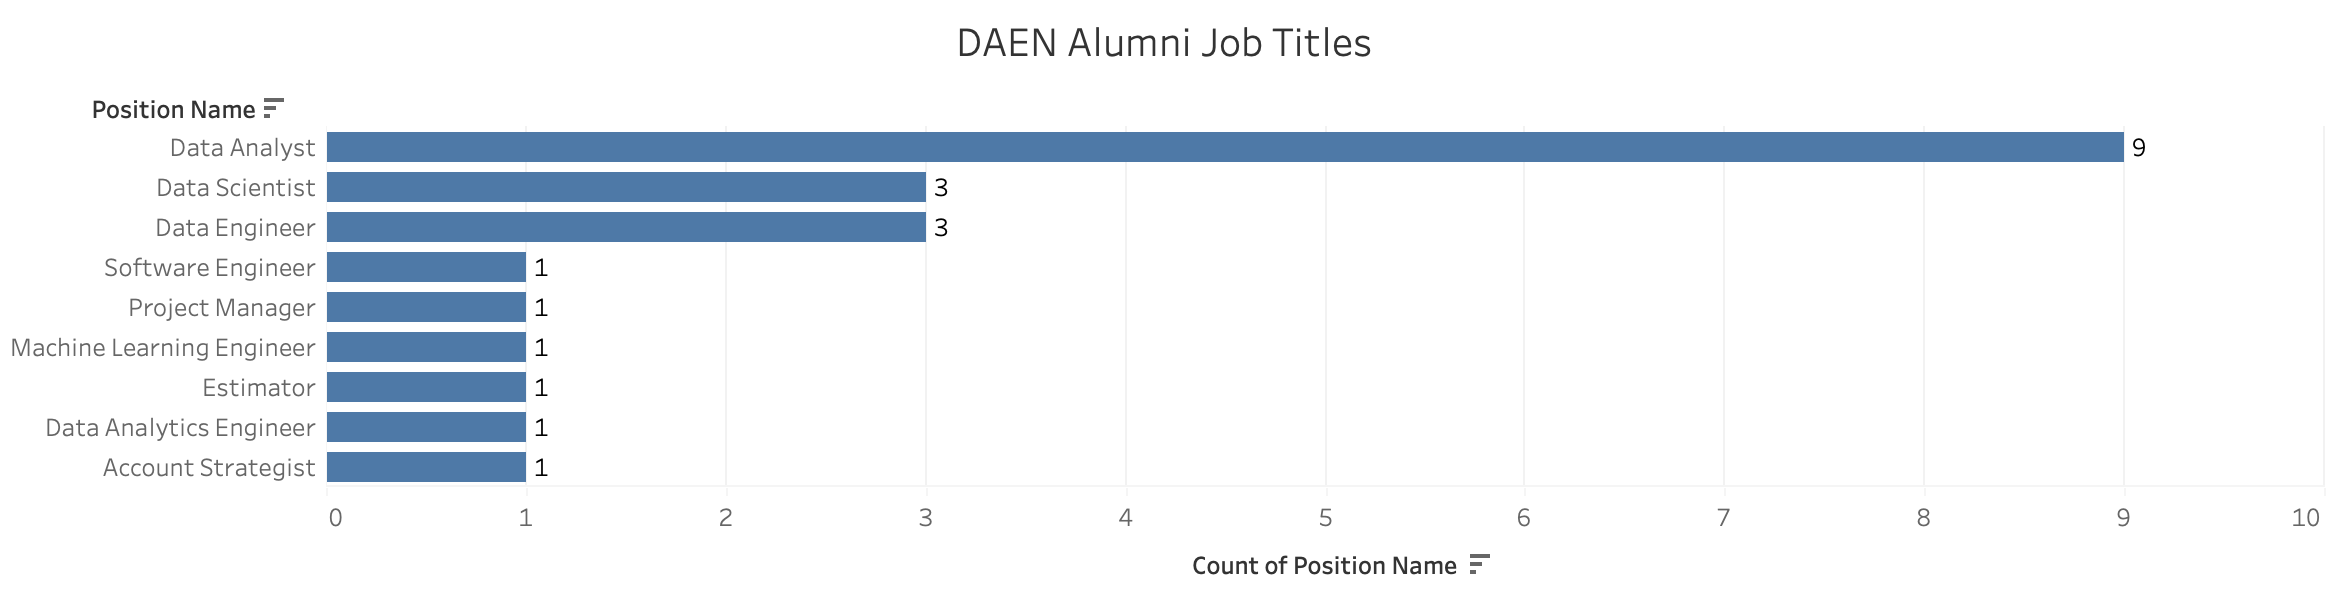
\includegraphics[width=0.9\textwidth]{visualizations/job-titles.png}
    \caption{Job Titles of DAEN Alumni}
    \label{fig:job-titles}
\end{figure}

The alumni job titles were consolidated, with roles like Business Analyst, Senior Data Analyst, and Lead Data Analyst grouped under "Data Analyst", which accounted for 43\% of jobs. This focused on core functions rather than seniority. Senior Data Scientist roles were similarly consolidated under the broader Data Scientist title.

\begin{figure}[H]
    \centering
    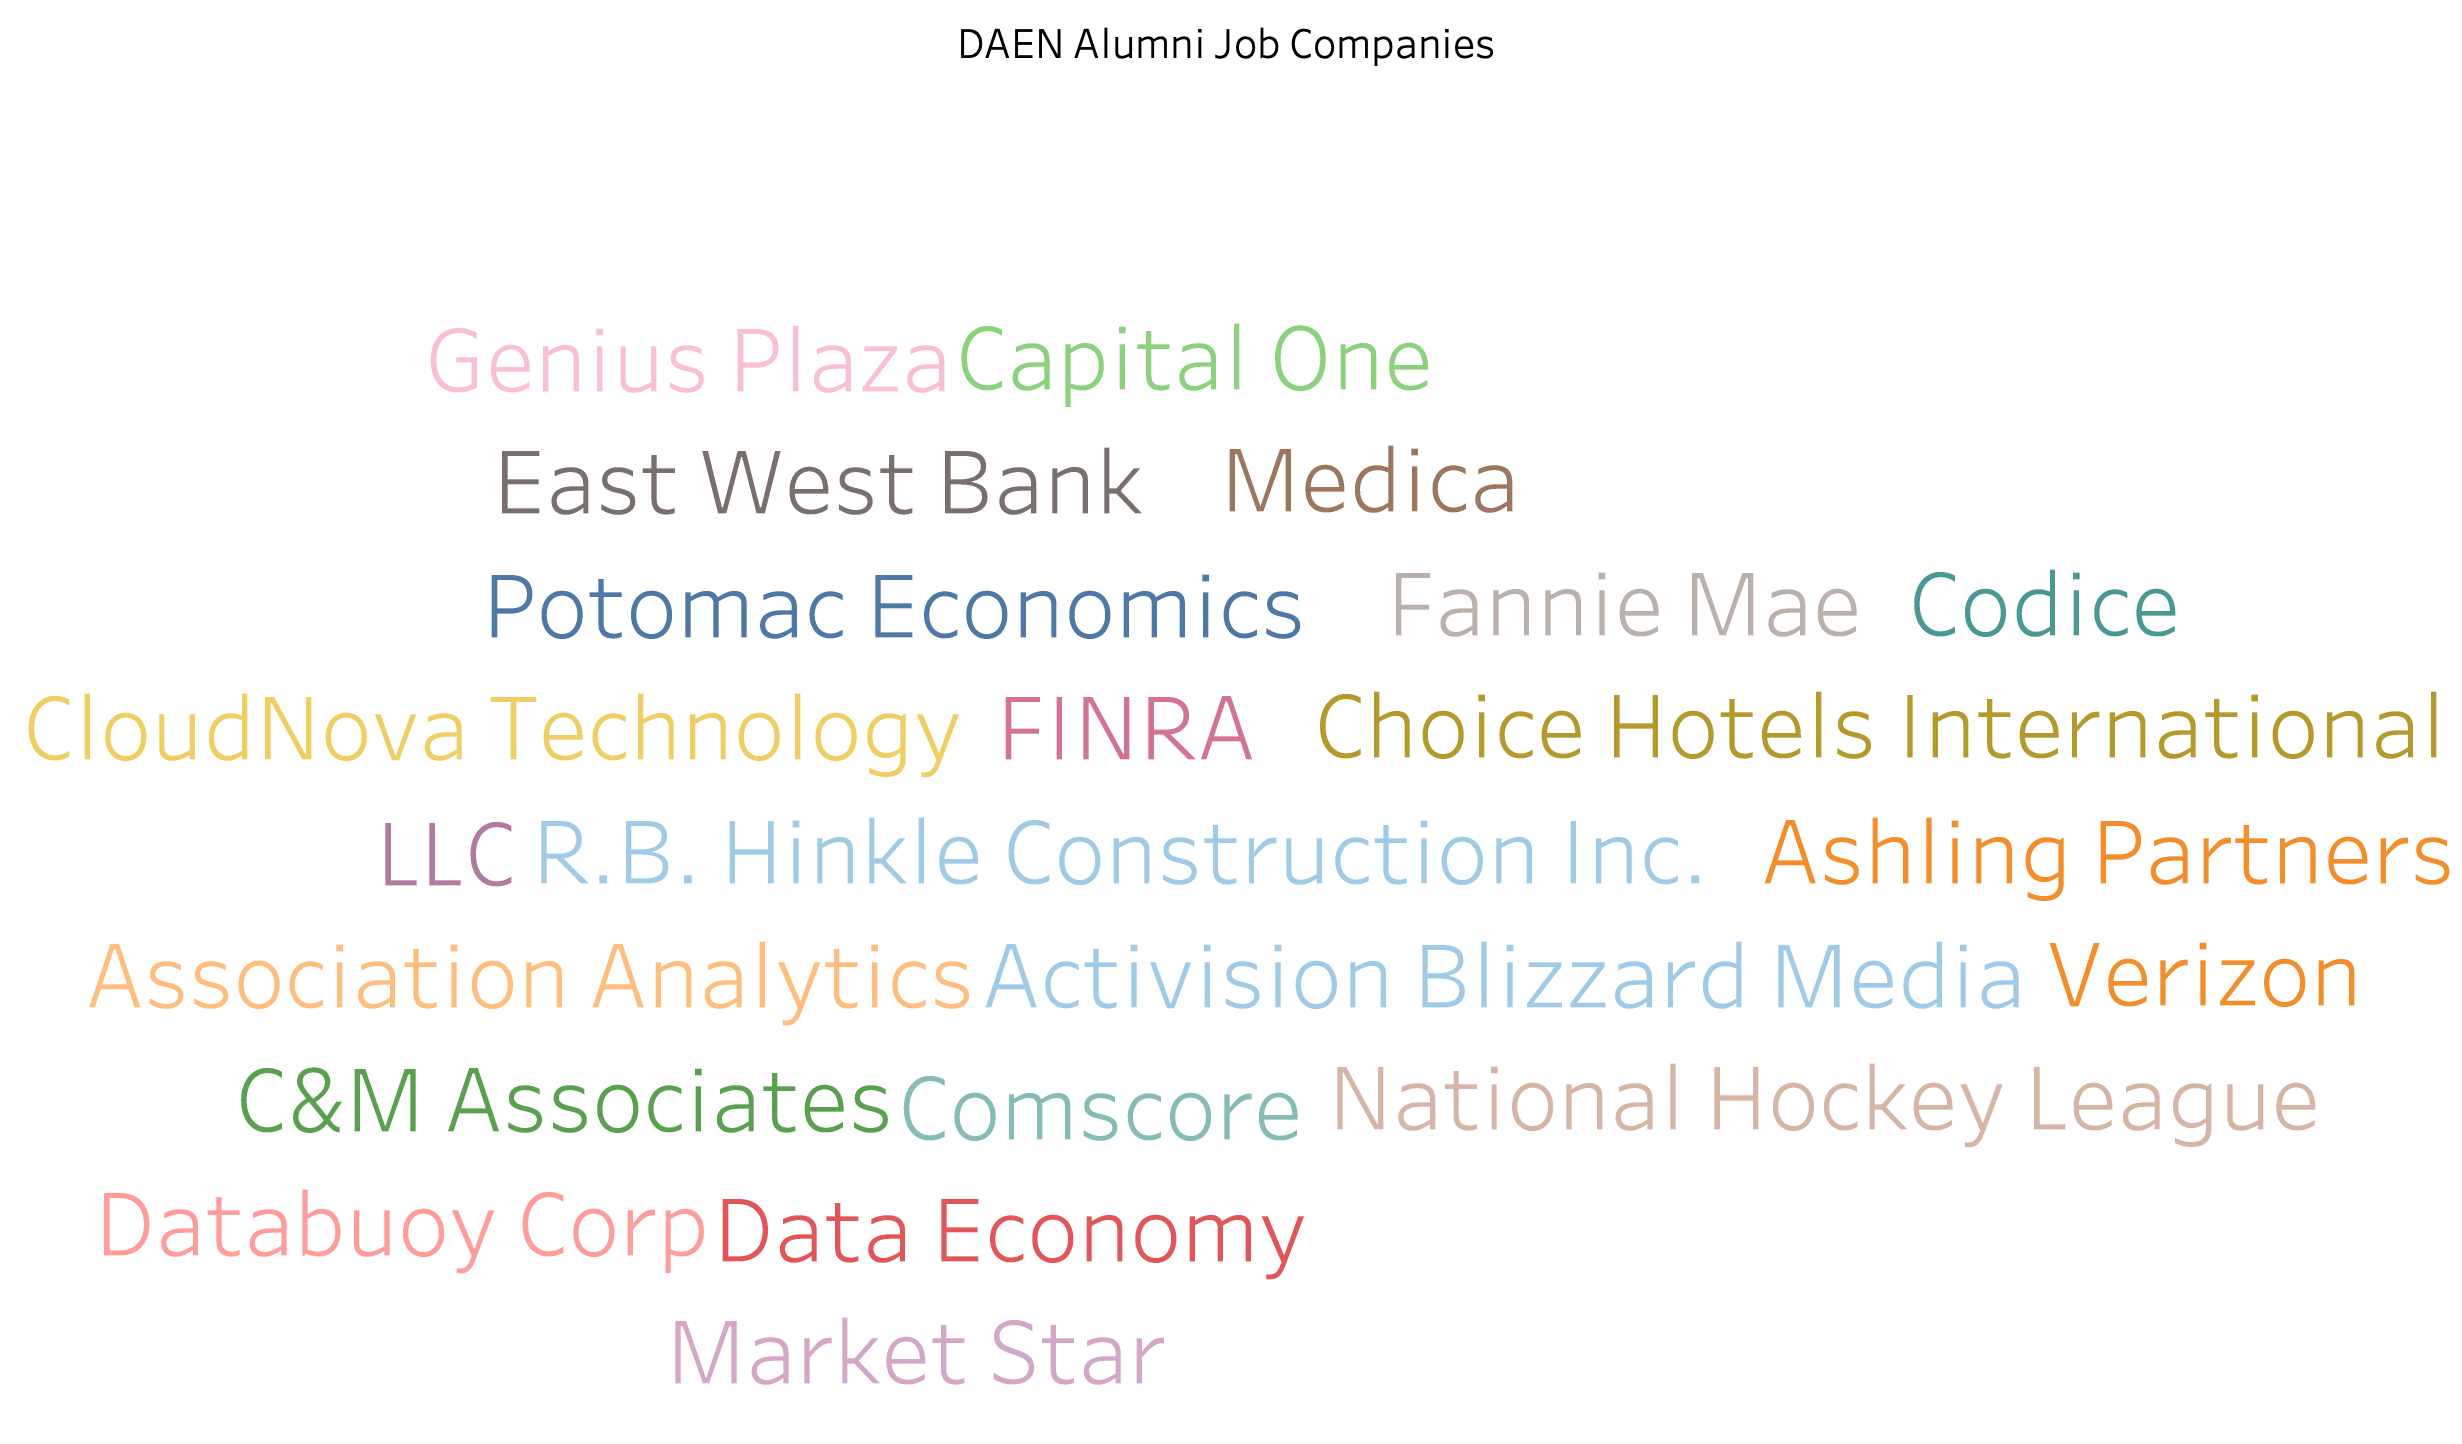
\includegraphics[width=0.9\textwidth]{visualizations/job-companies.png}
    \caption{Companies Employing DAEN Alumni}
    \label{fig:job-companies}
\end{figure}

The diversity in employing companies demonstrates broad industry recognition of the program, with no single industry dominating employment outcomes. 

\begin{figure}[H]
    \centering
    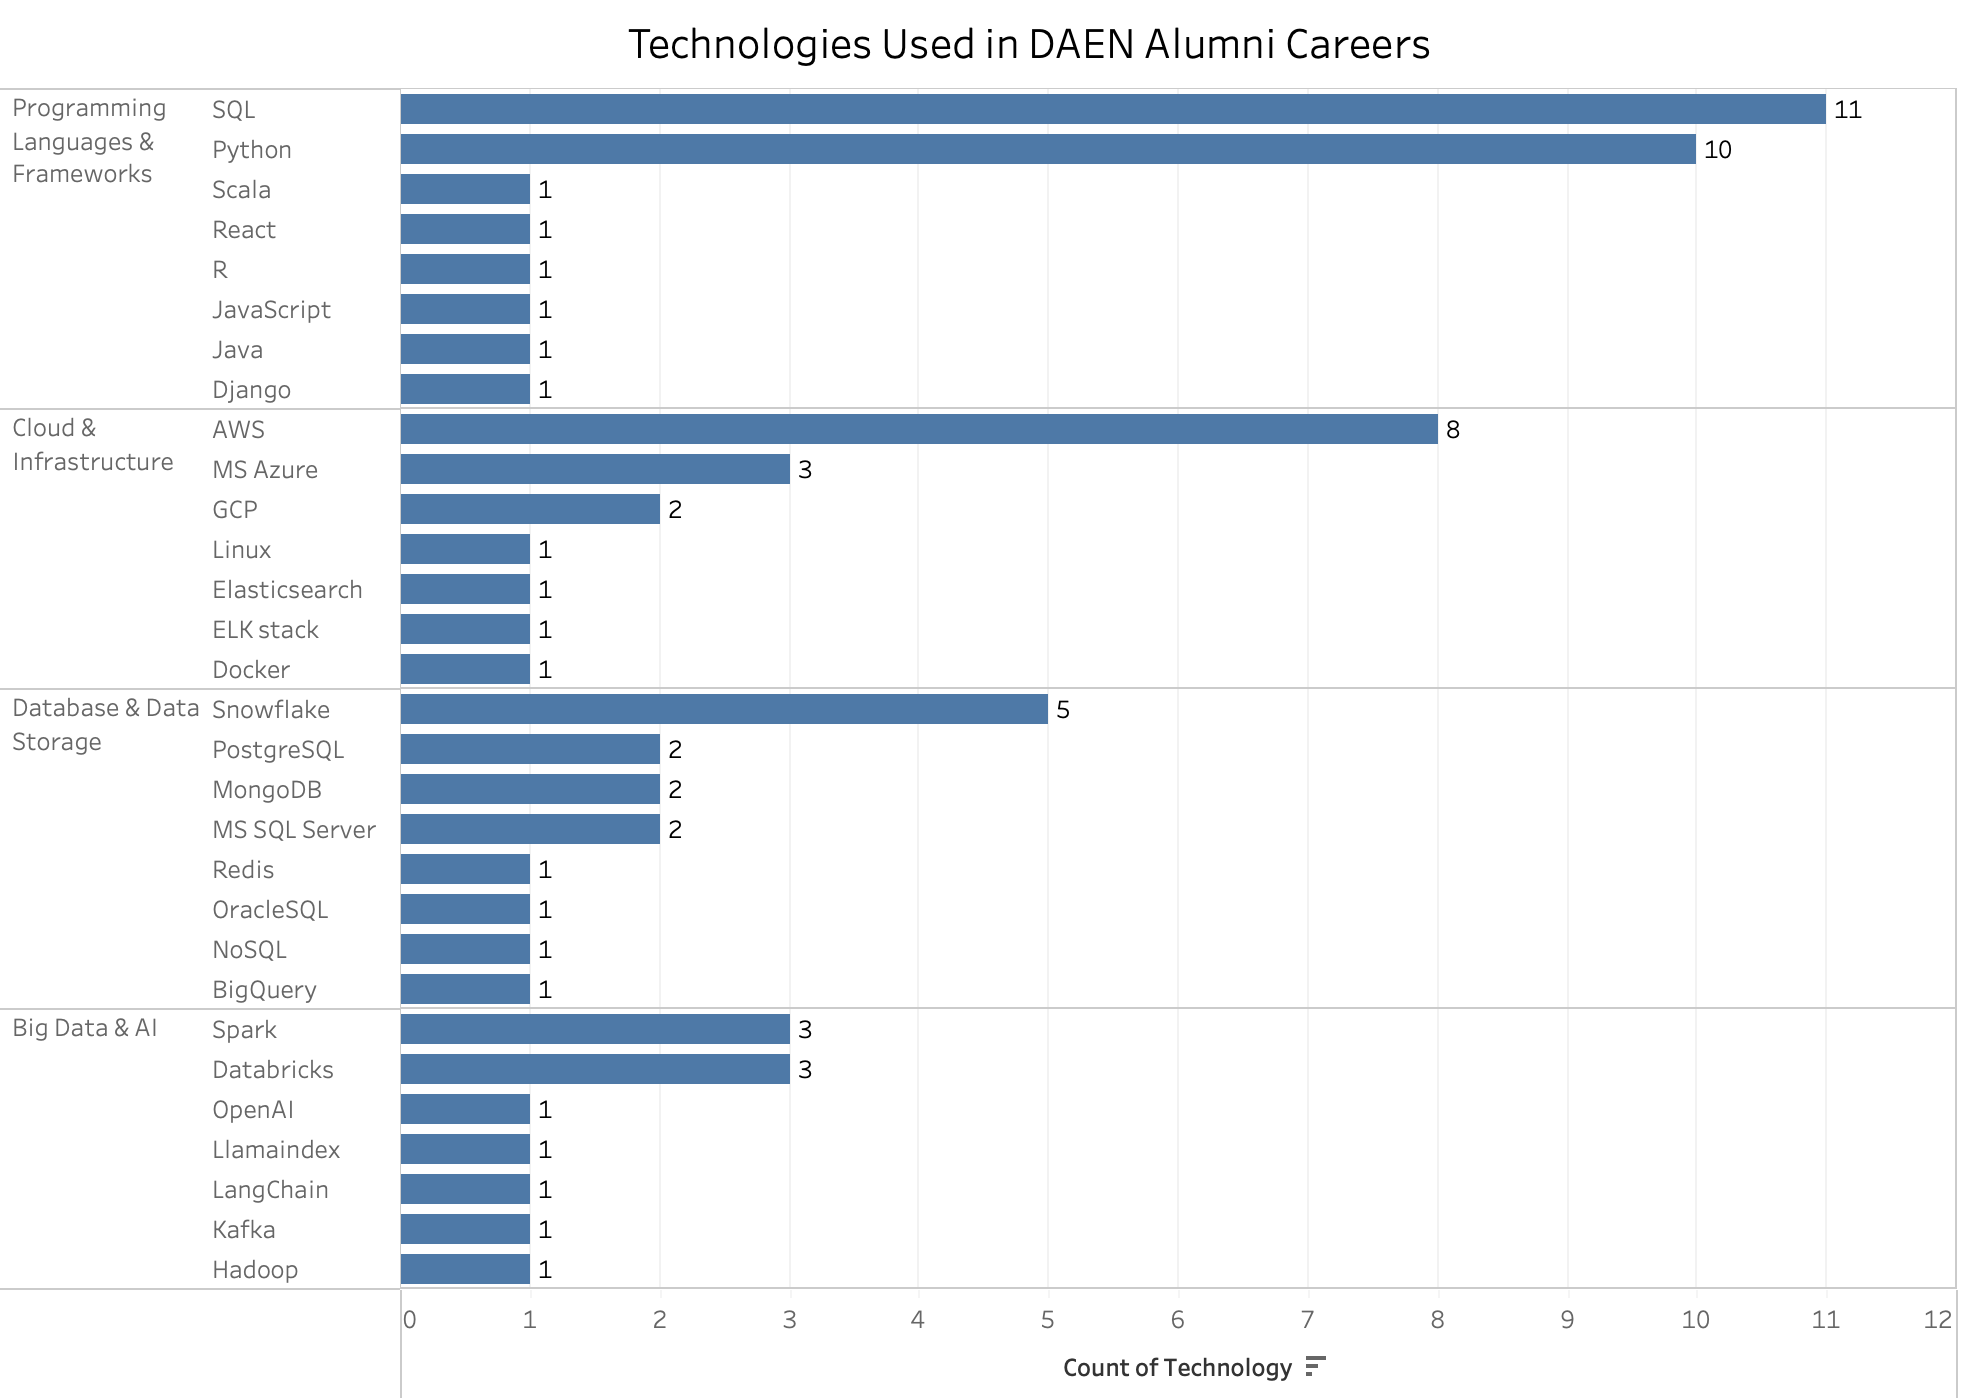
\includegraphics[width=0.9\textwidth]{visualizations/career-technologies.png}
    \caption{Technologies Used in DAEN Alumni Careers}
    \label{fig:career-technologies}
\end{figure}

Technology usage shows clear patterns:
\begin{itemize}
\item Programming Languages \& Frameworks: Python and SQL dominate (78\% usage)
\item Cloud \& Infrastructure: AWS leads with 47\% adoption
\item Database \& Data Storage: Snowflake is increasingly popular (33\% usage)
\item Big Data \& AI: Spark and Databricks (55\% usage)
\end{itemize}

\begin{figure}[H]
    \centering
    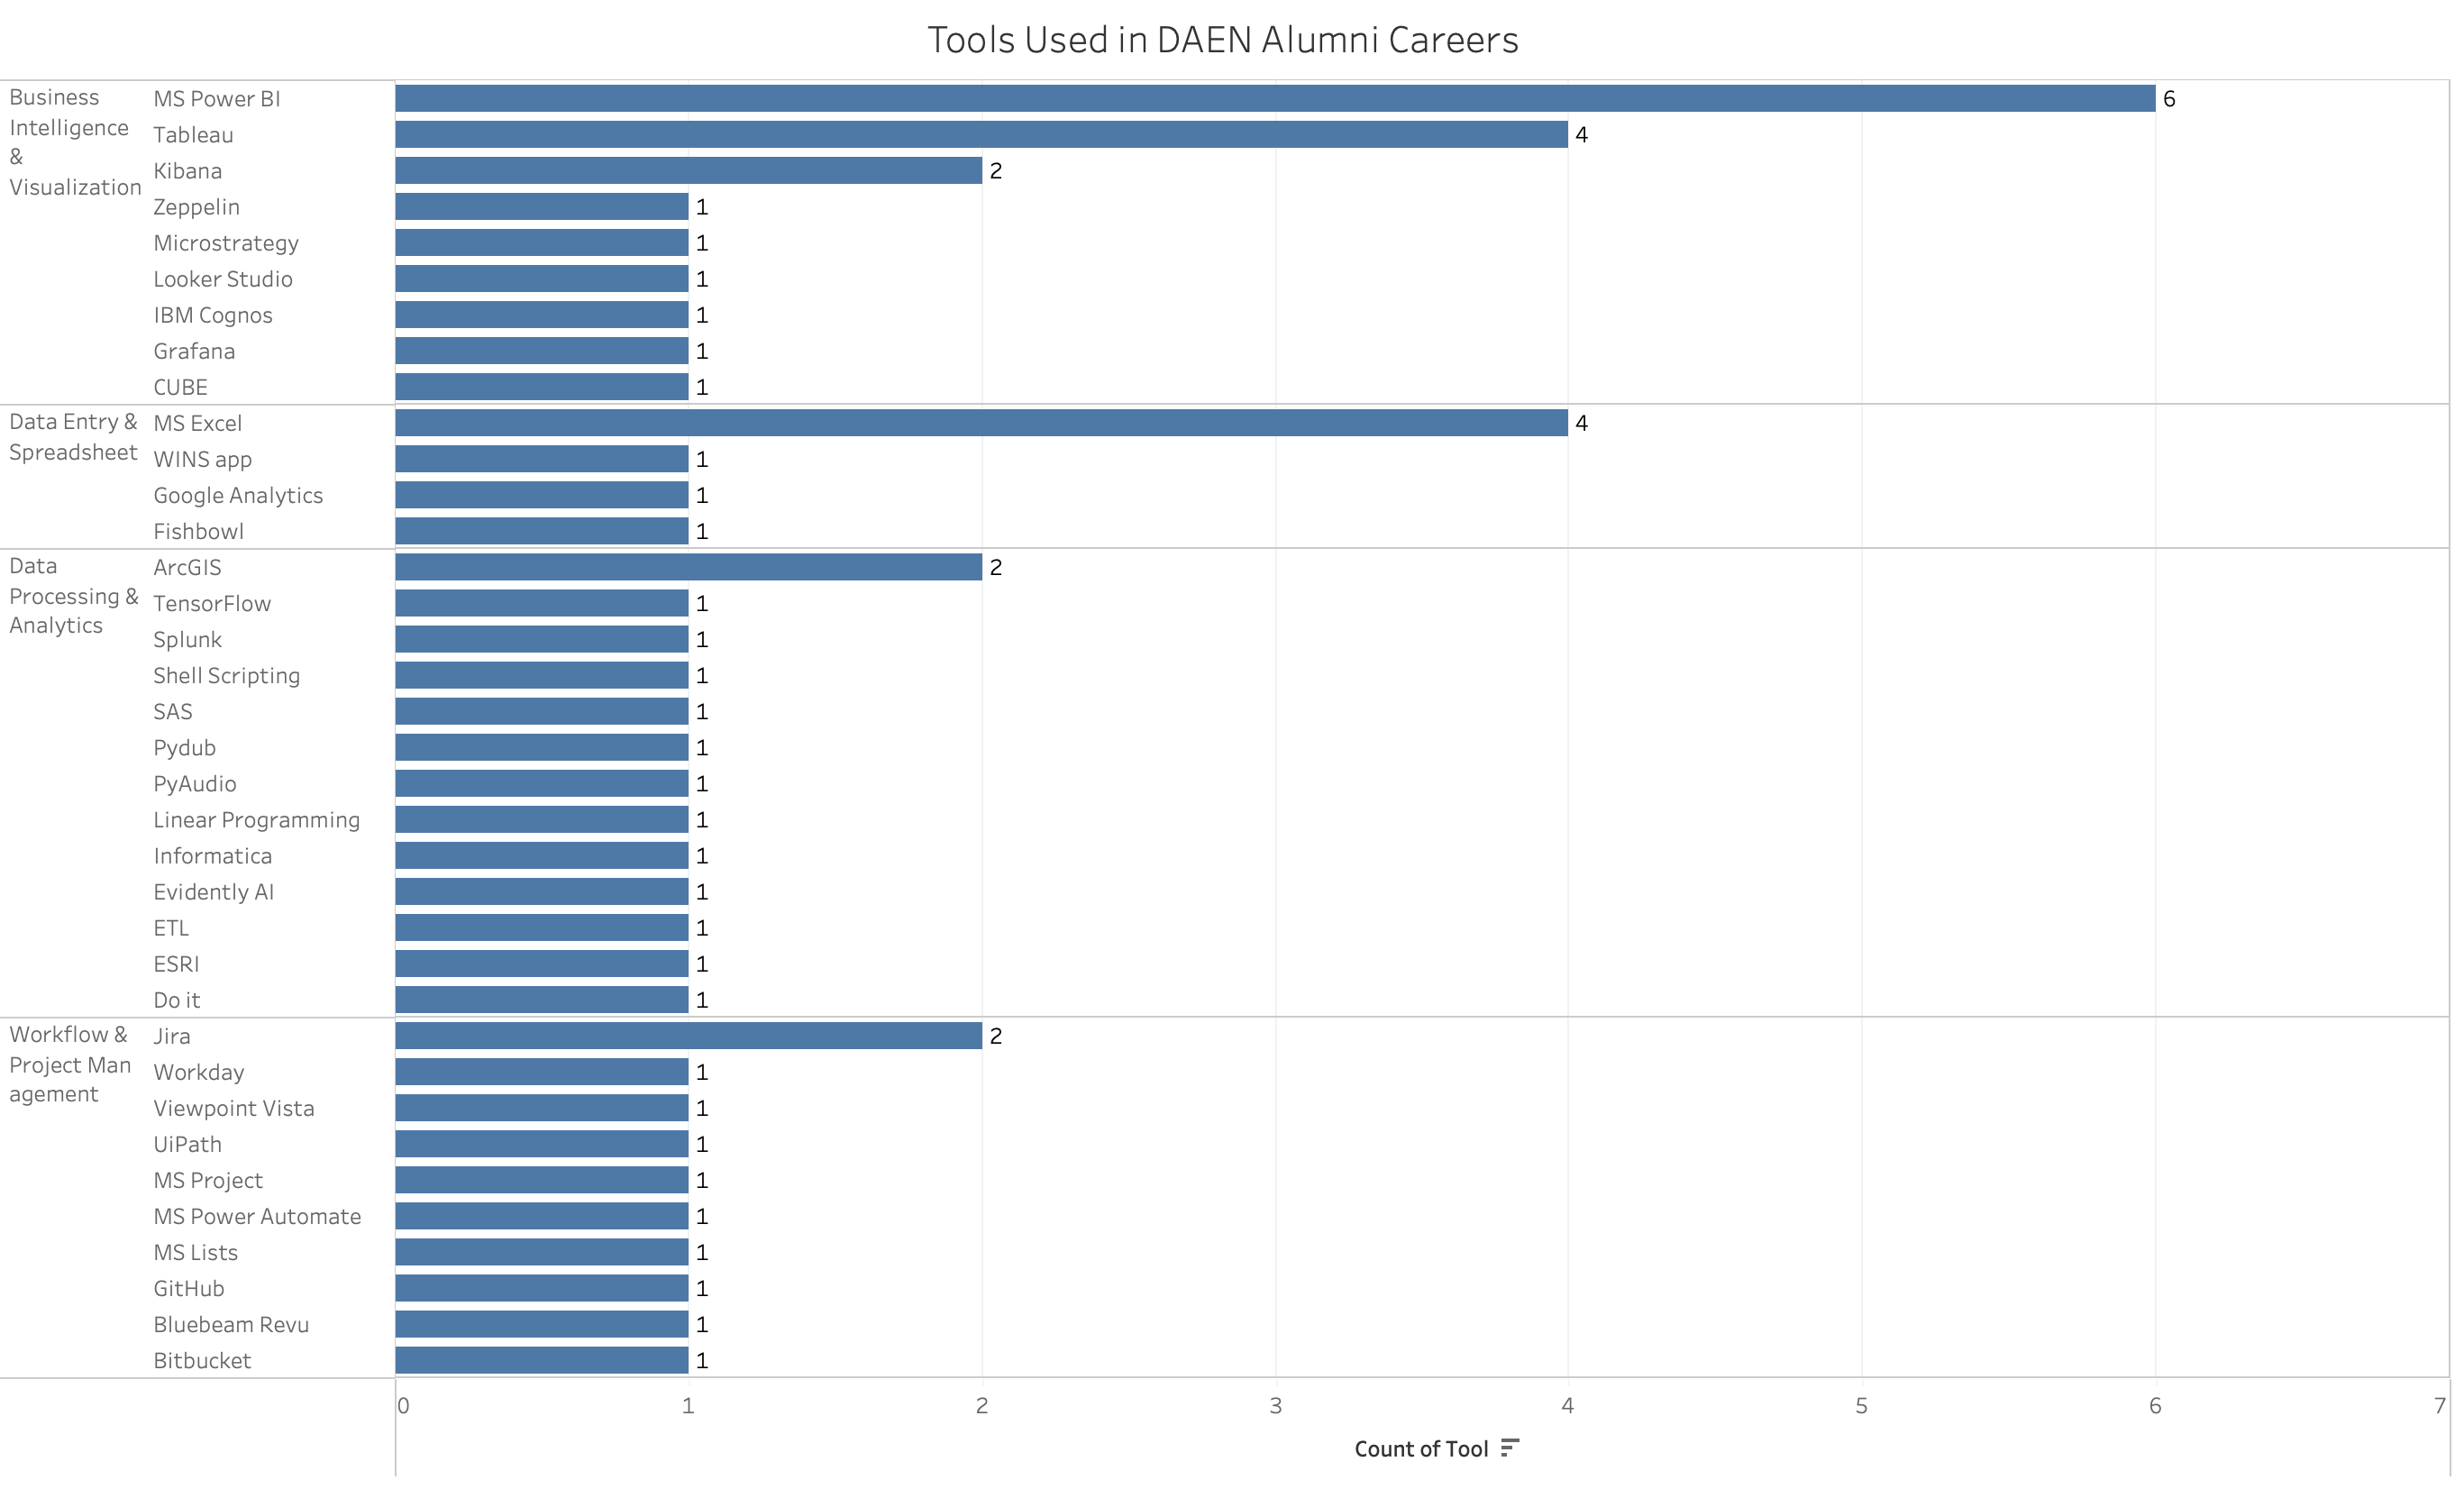
\includegraphics[width=0.9\textwidth]{visualizations/career-tools.png}
    \caption{Tools Used in DAEN Alumni Careers}
    \label{fig:career-tools}
\end{figure}

Visualization and analytics tools show strong preferences:
\begin{itemize}
\item Business Intelligence \& Visualization: Power BI and Tableau lead adoption
\item Data Entry \& Spreadsheet: Heavy use of MS Excel
\item Data Processing \& Analytics: Popular in ArcGIS
\item Workflow \& Project Management: Popular in Jira
\end{itemize}
\begin{figure}[H]
    \centering
    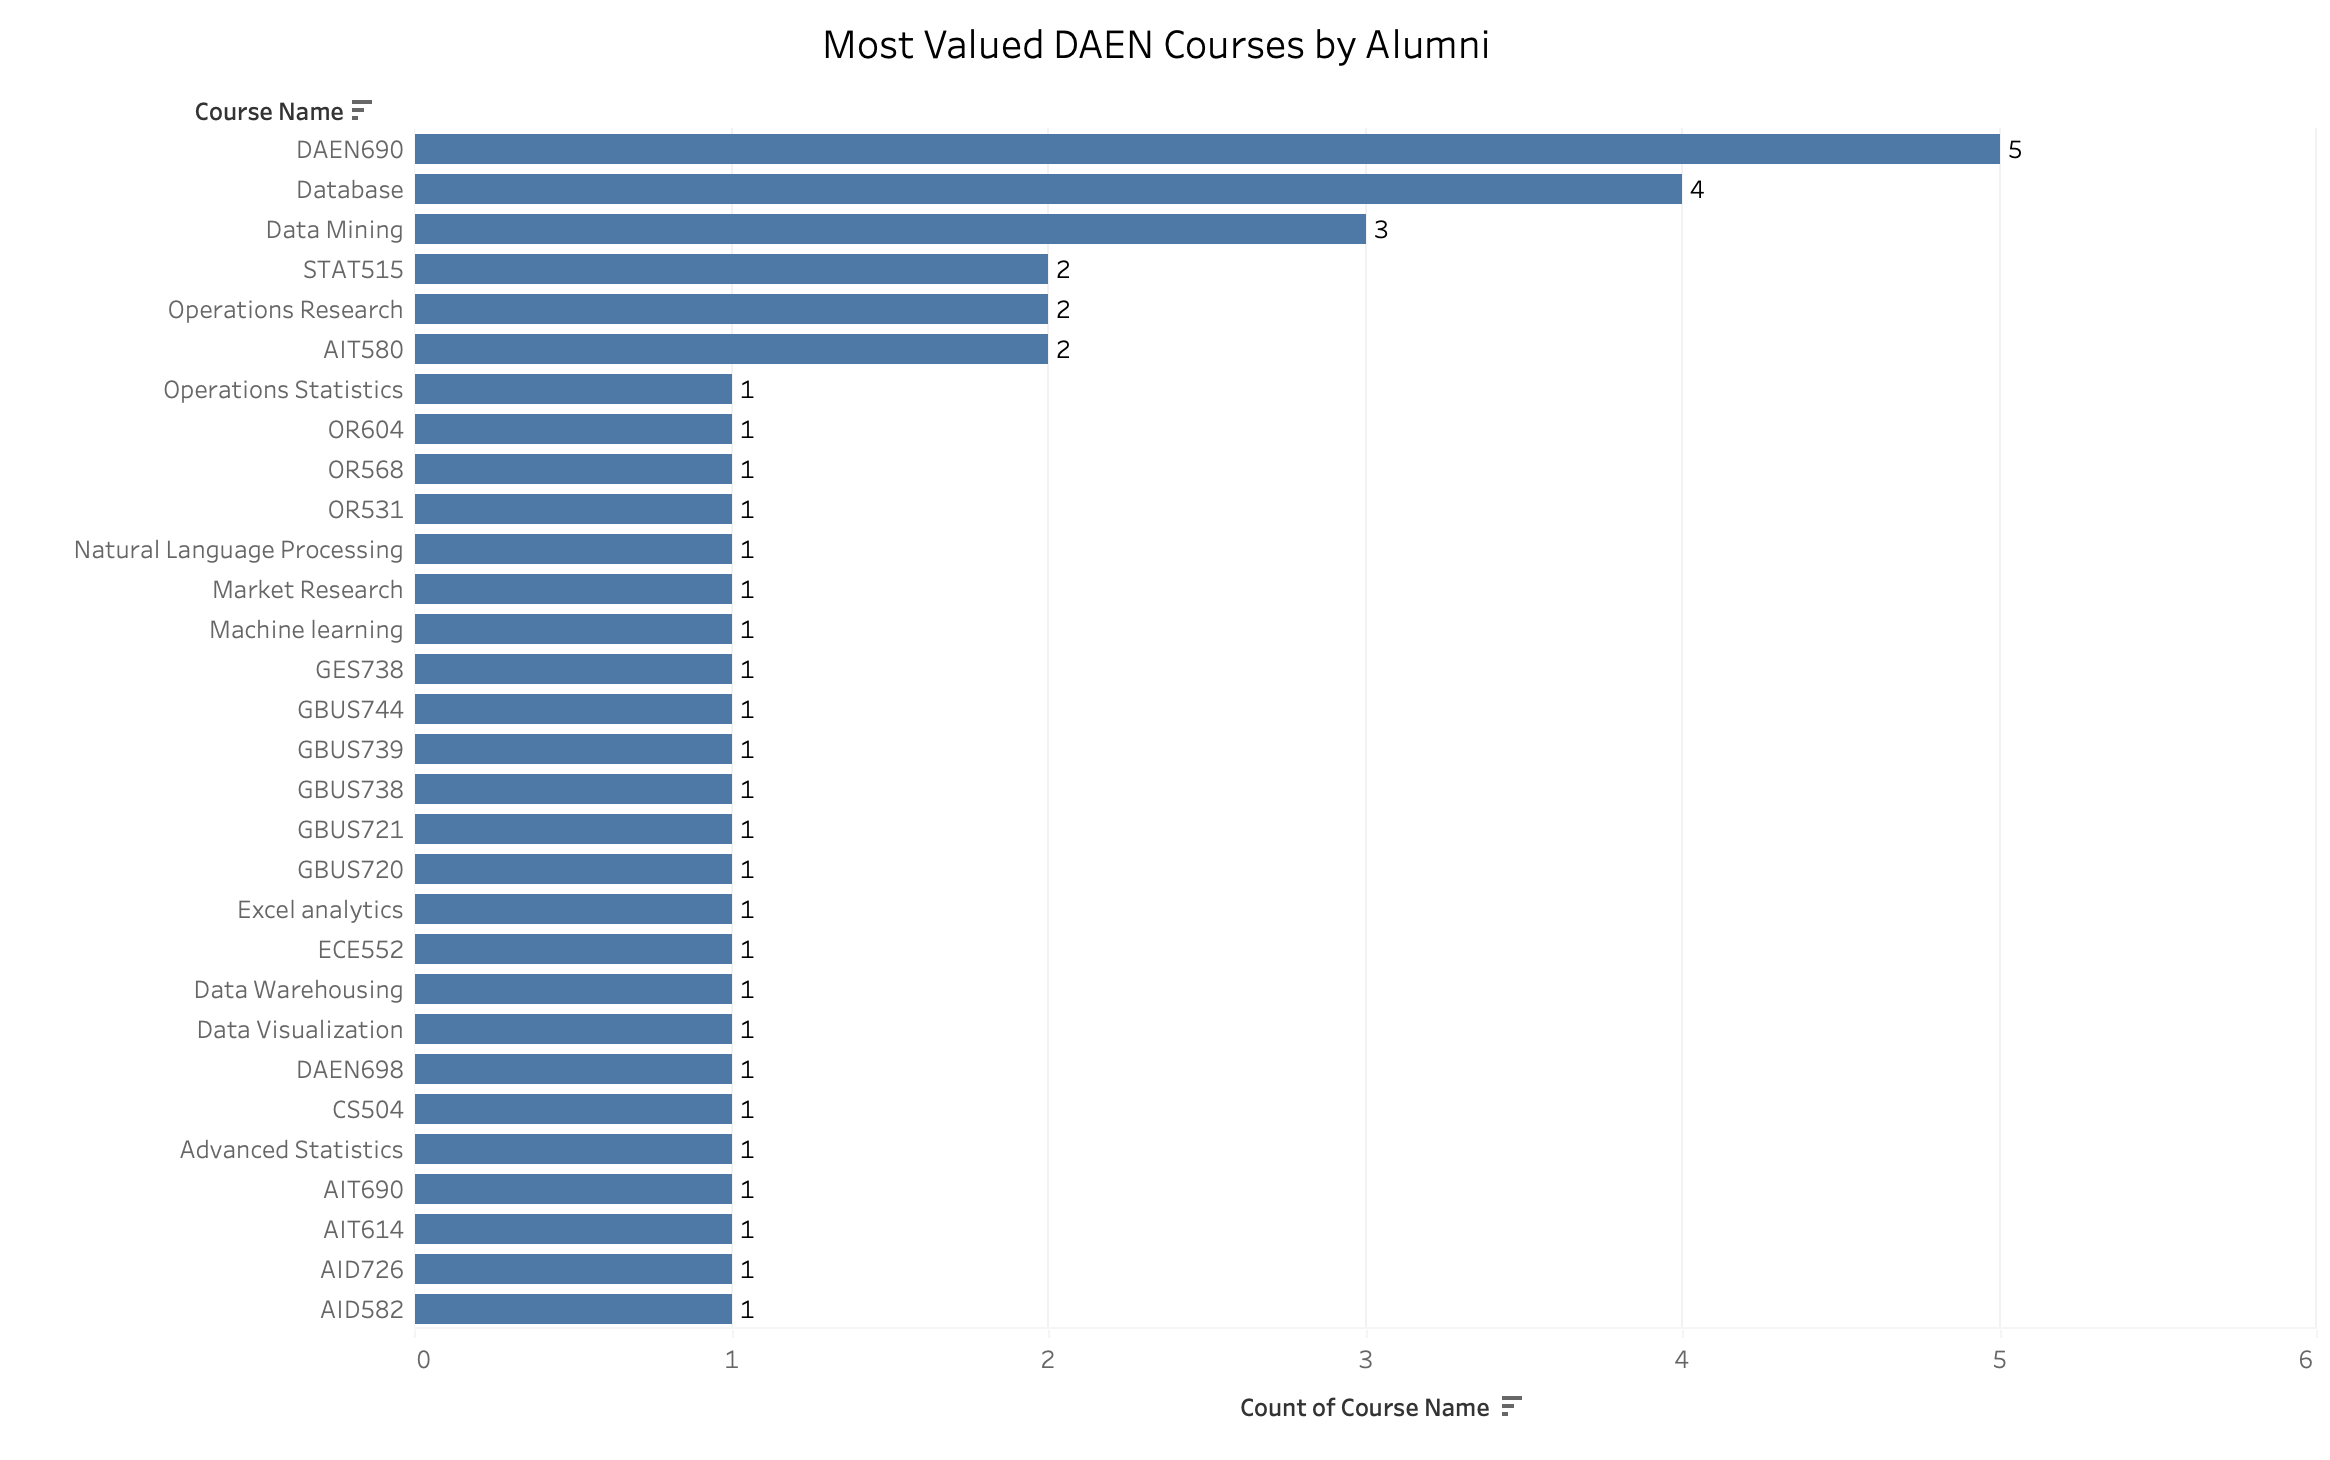
\includegraphics[width=0.9\textwidth]{visualizations/daen-courses.png}
    \caption{Valuable Program Courses}
    \label{fig:daen-courses}
\end{figure}

Course evaluations highlight key program strengths:
\begin{itemize}
\item DAEN 690, Data Analytics Project (Capstone course)
\item Database courses
\item Required DAEN core courses showed strong practical value (AIT 580, Data Mining, STAT 515, Operations Research, AND DAEN 690)
\end{itemize}
\begin{figure}[H]
    \centering
    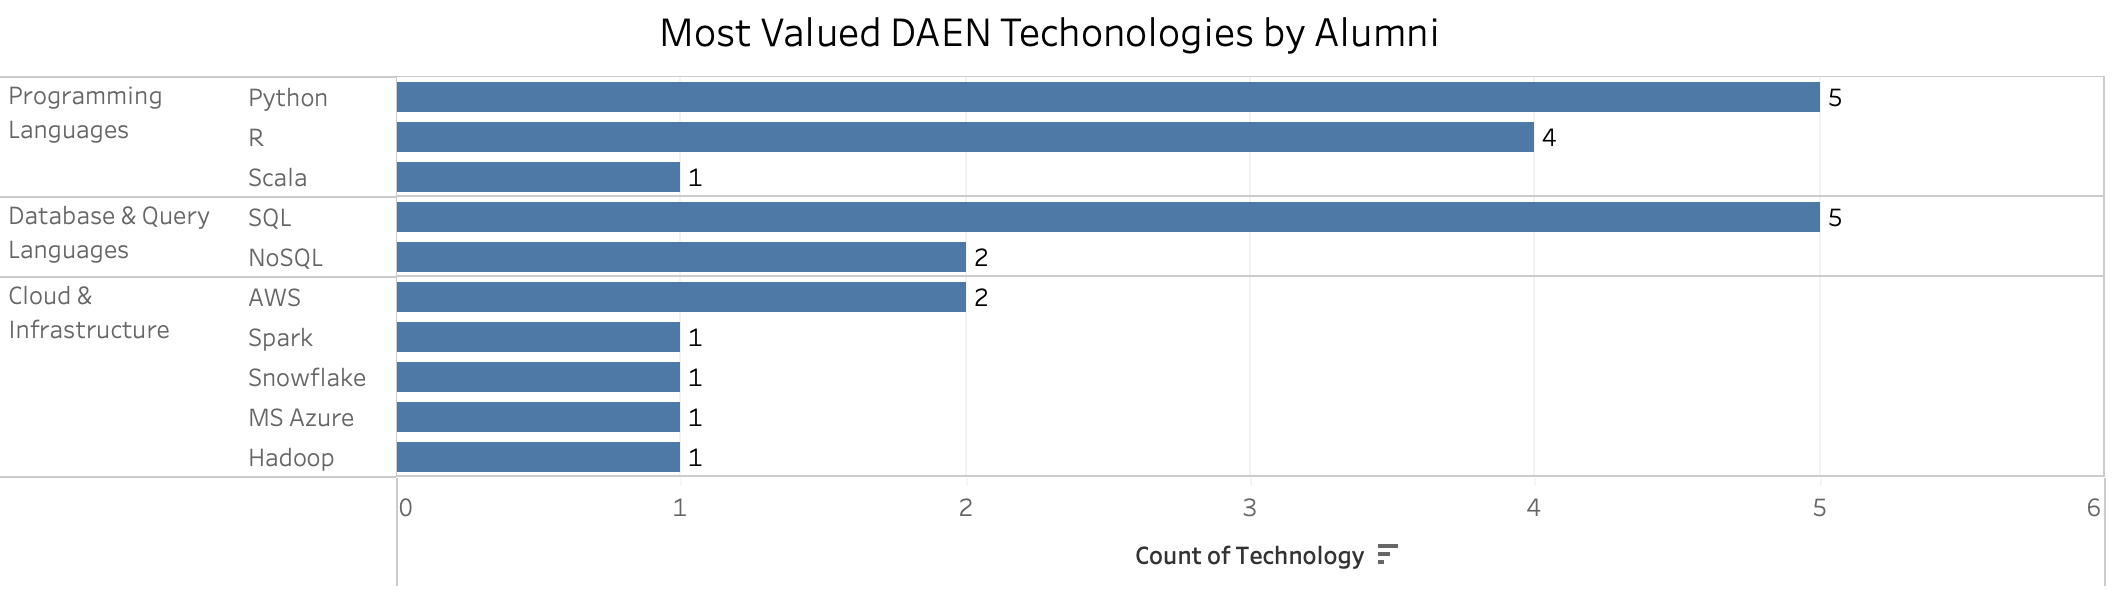
\includegraphics[width=0.9\textwidth]{visualizations/daen-technologies.png}
    \caption{Valuable Technologies Acquired in DAEN Program}
    \label{fig:daen-technologies}
\end{figure}

SQL and Python emerge as the most beneficial technologies learned, aligning well with industry demands as the most commonly used technologies in DAEN alumni careers.

\begin{figure}[H]
    \centering
    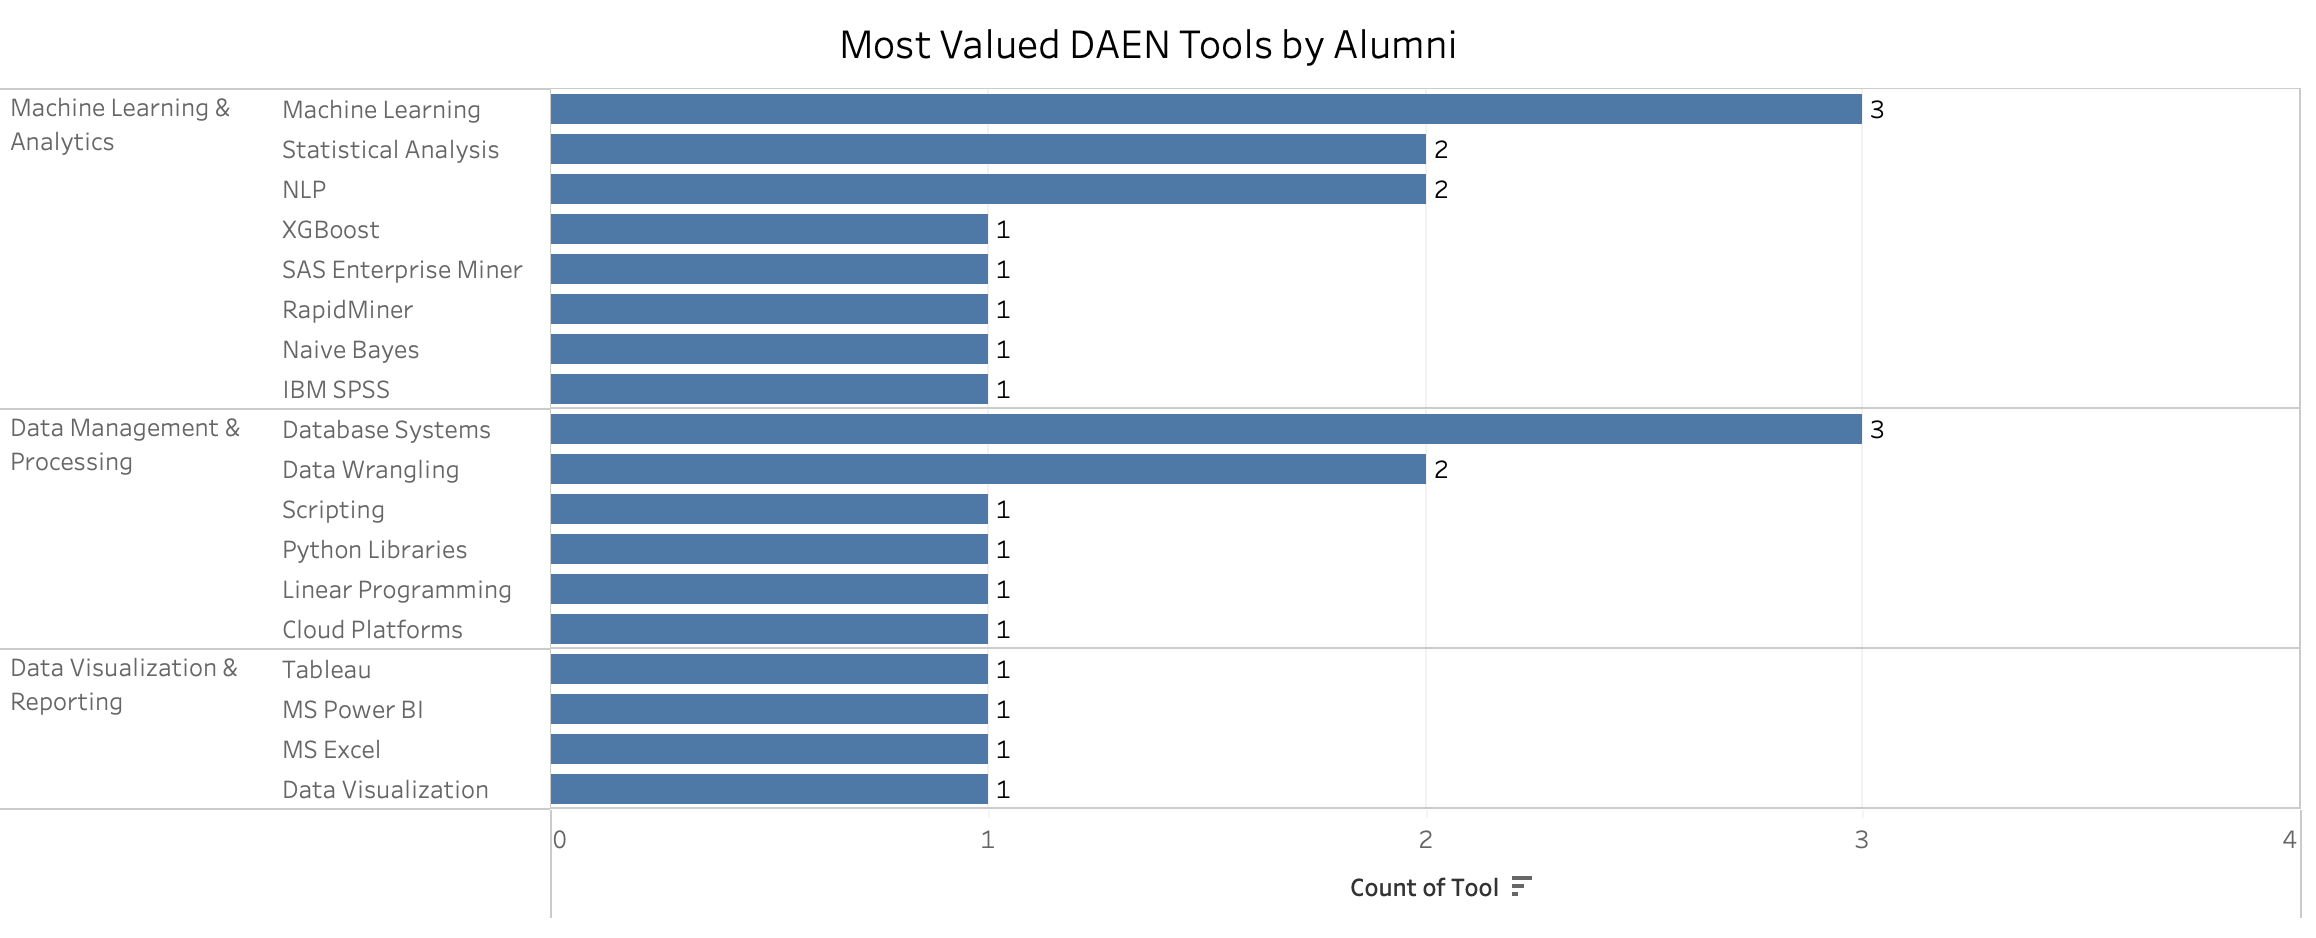
\includegraphics[width=0.9\textwidth]{visualizations/daen-tools.png}
    \caption{Valuable Tools Acquired in DAEN Program}
    \label{fig:daen-tools}
\end{figure}

Machine learning and database systems emerged as the most valuable tools acquired from the program.

\begin{figure}[H]
    \centering
    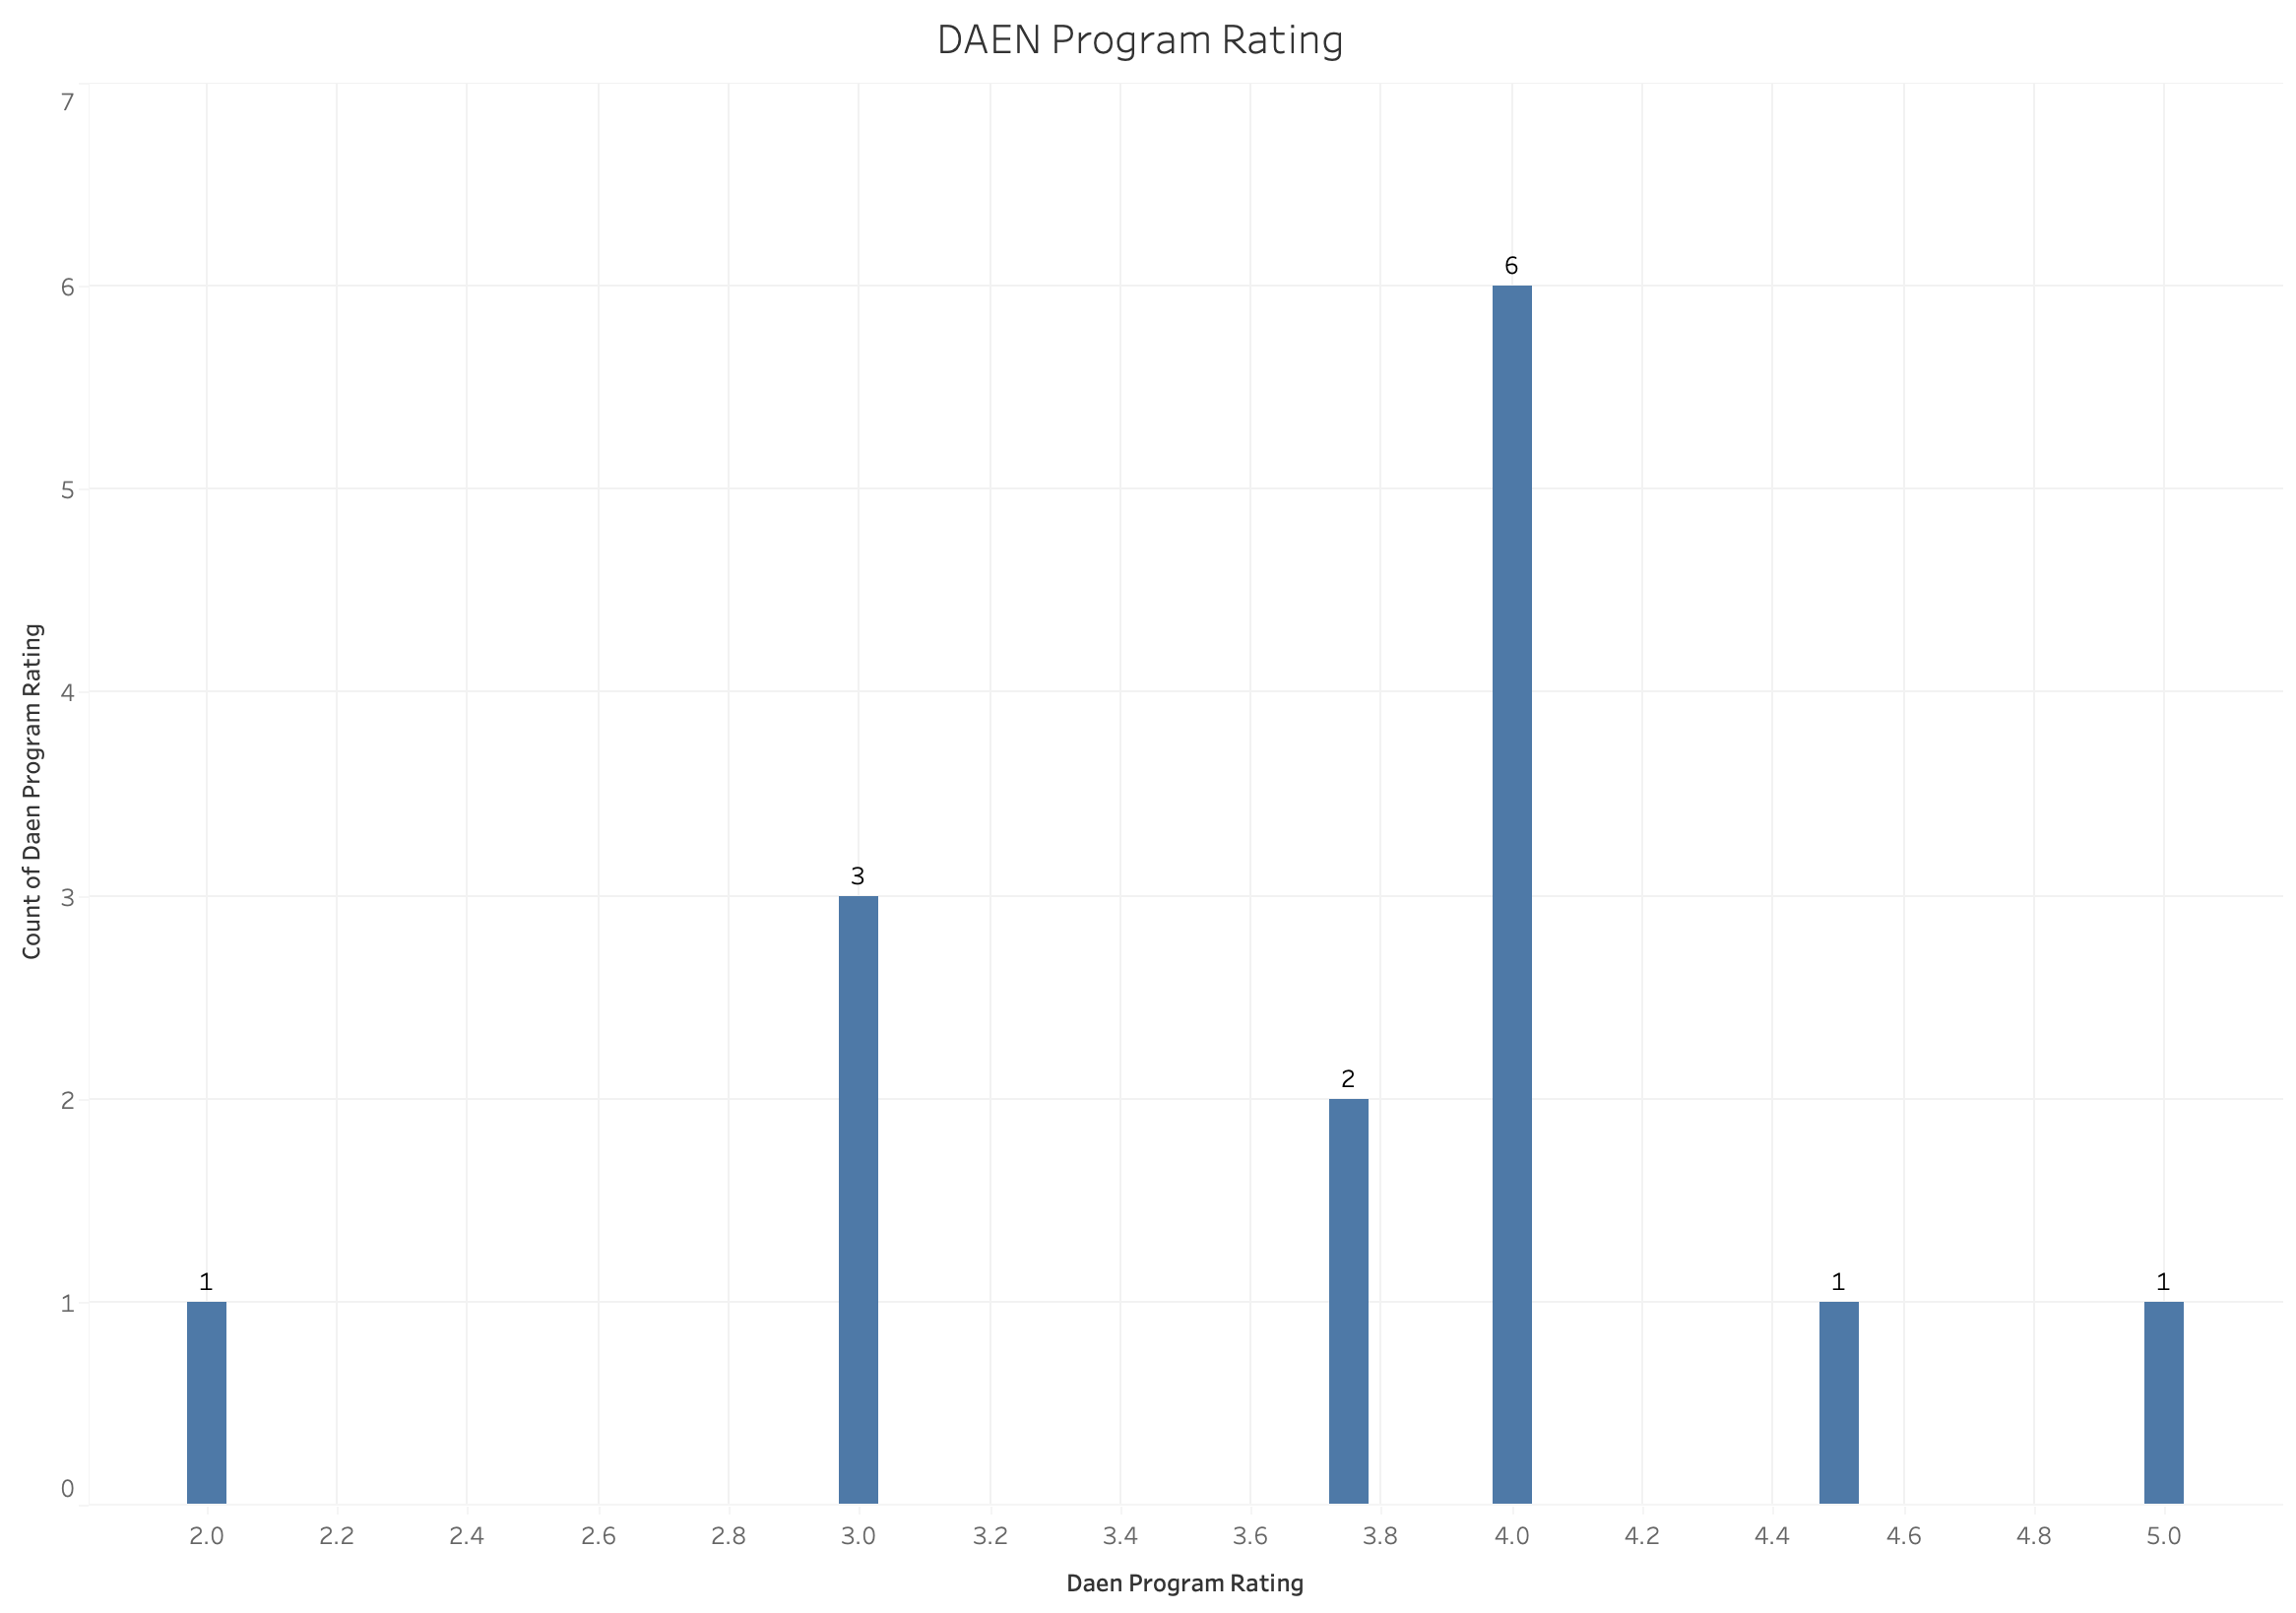
\includegraphics[width=0.9\textwidth]{visualizations/daen-rating.png}
    \caption{DAEN Alumni Program Ratings}
    \label{fig:daen-rating}
\end{figure}

The program received an average rating of 3.7 out of 5, with most alumni rating it 4 out of 5. This indicates relatively high satisfaction with their education while also suggesting areas for potential improvement.

\begin{figure}[H]
    \centering
    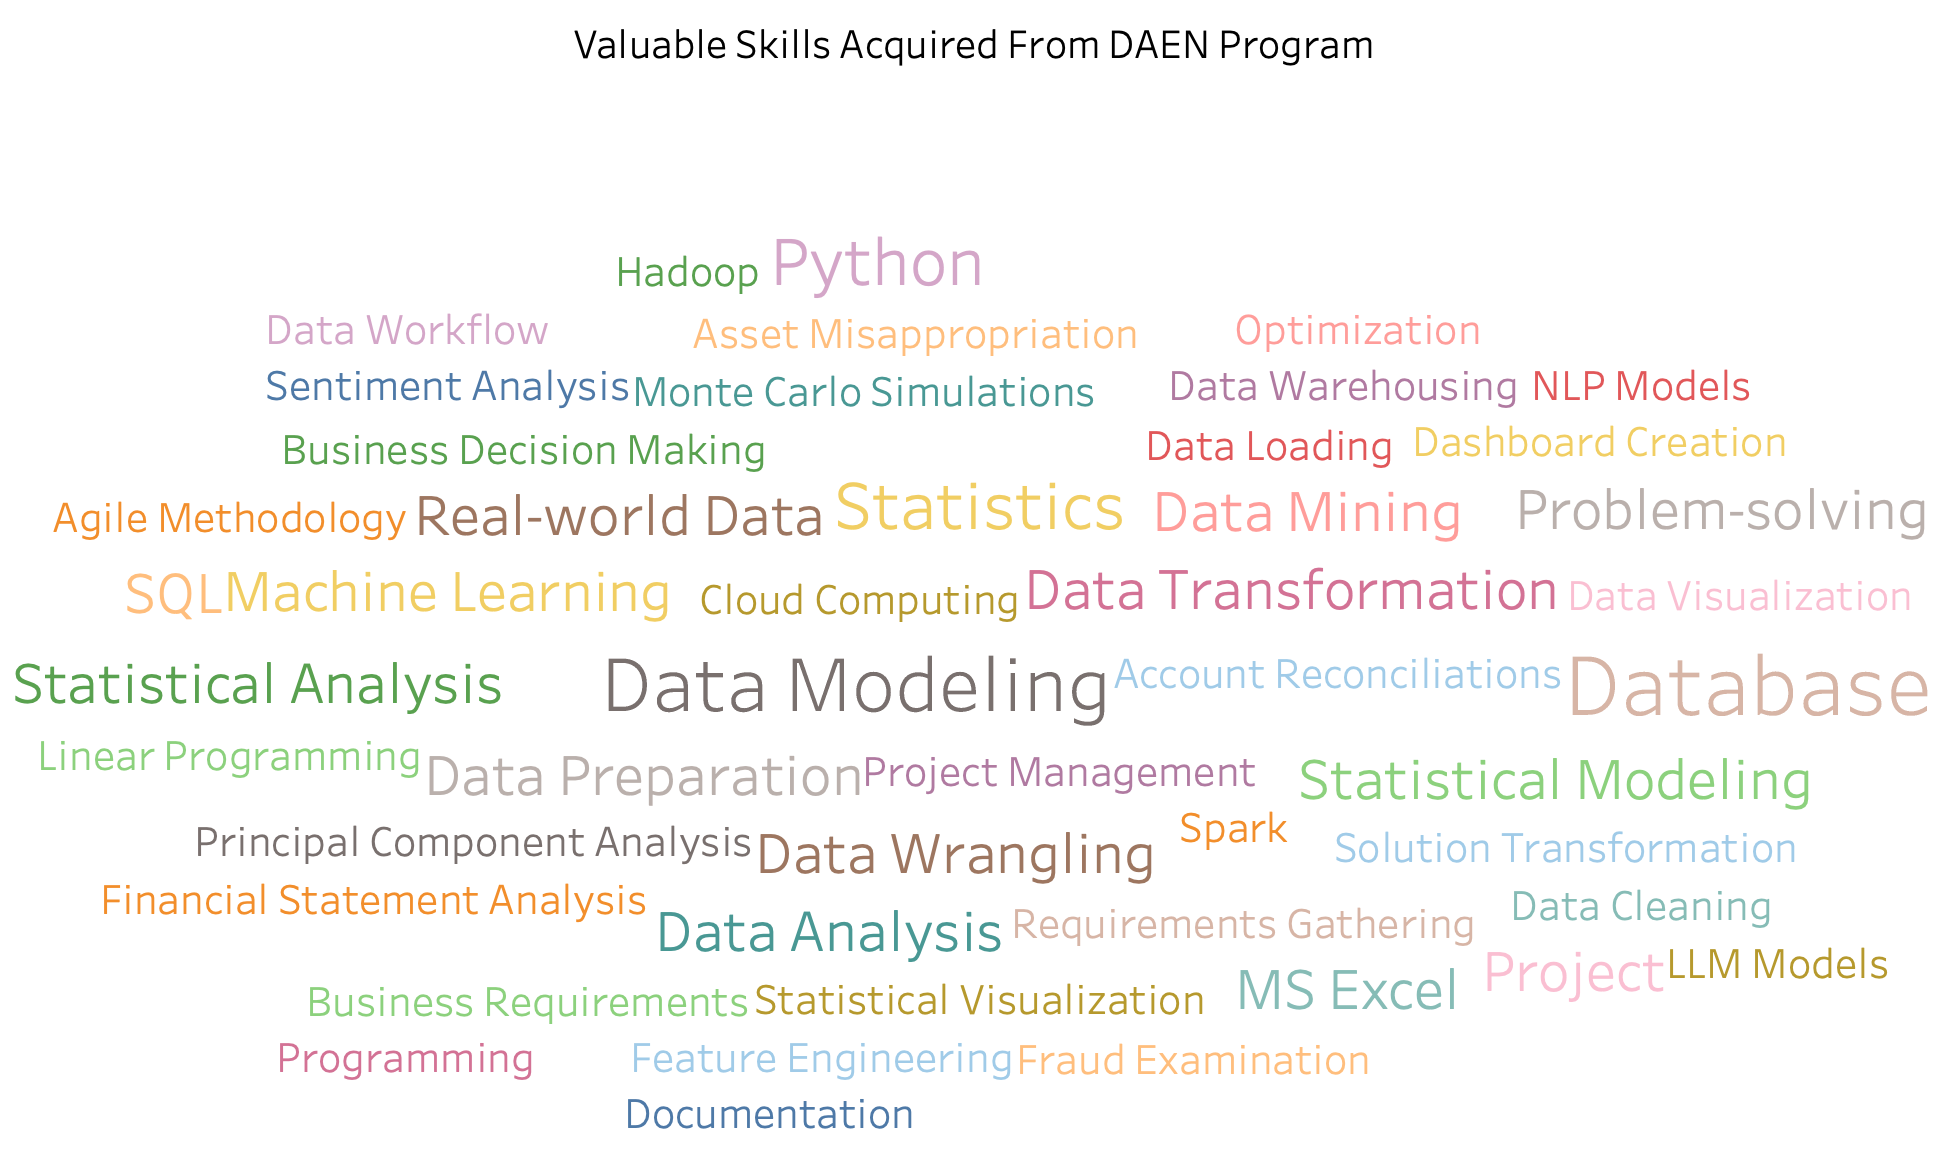
\includegraphics[width=0.9\textwidth]{visualizations/program-skills.png}
    \caption{Valuable Skills Acquired in DAEN Program}
    \label{fig:program-skills}
\end{figure}

Alumni particularly valued data modeling and database skills gained from the program. The emphasis on database systems and machine learning concepts appears to align well with industry needs. 

\begin{figure}[H]
    \centering
    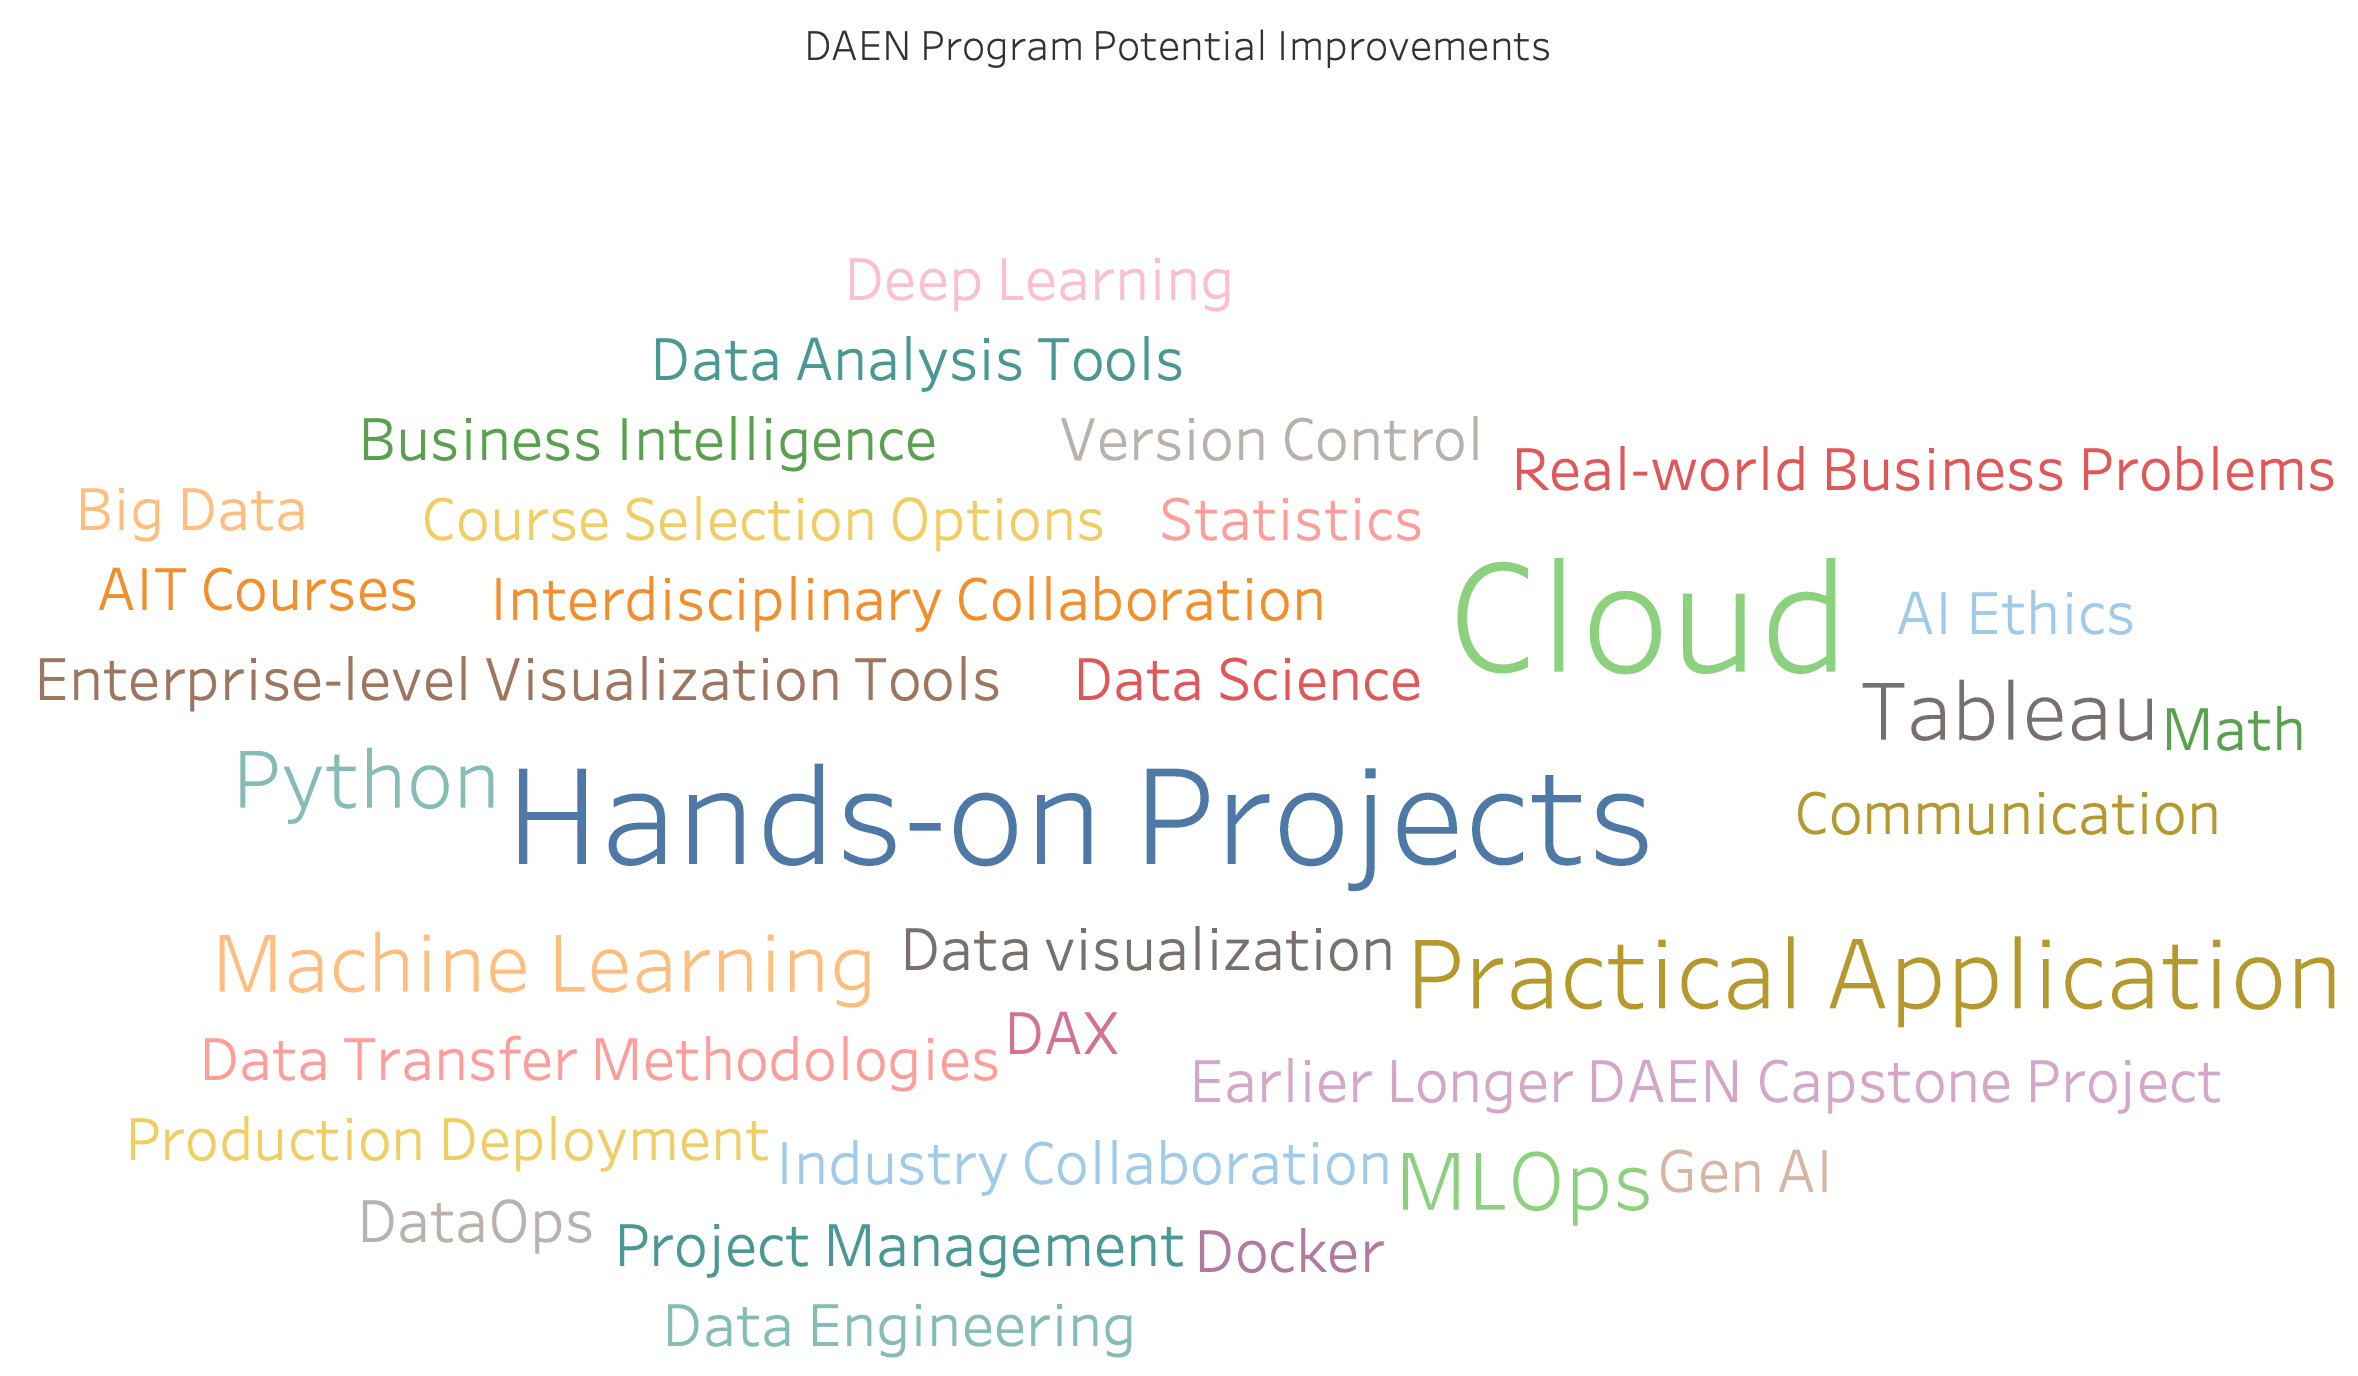
\includegraphics[width=0.9\textwidth]{visualizations/potential-improvements.png}
    \caption{Potential Program Improvements Suggested by Alumni}
    \label{fig:potential-improvements}
\end{figure}

Three main areas for improvement emerged from alumni feedback:
\begin{itemize}
\item Increased emphasis on cloud computing technologies, particularly AWS as many alumni use cloud in their roles and received limited exposure during their coursework
\item More hands-on project opportunities
\item Enhanced coverage of emerging technologies
\end{itemize}

These suggestions reflect the evolving needs of the industry and the gap between academic training and professional requirements.

\begin{figure}[H]
    \centering
    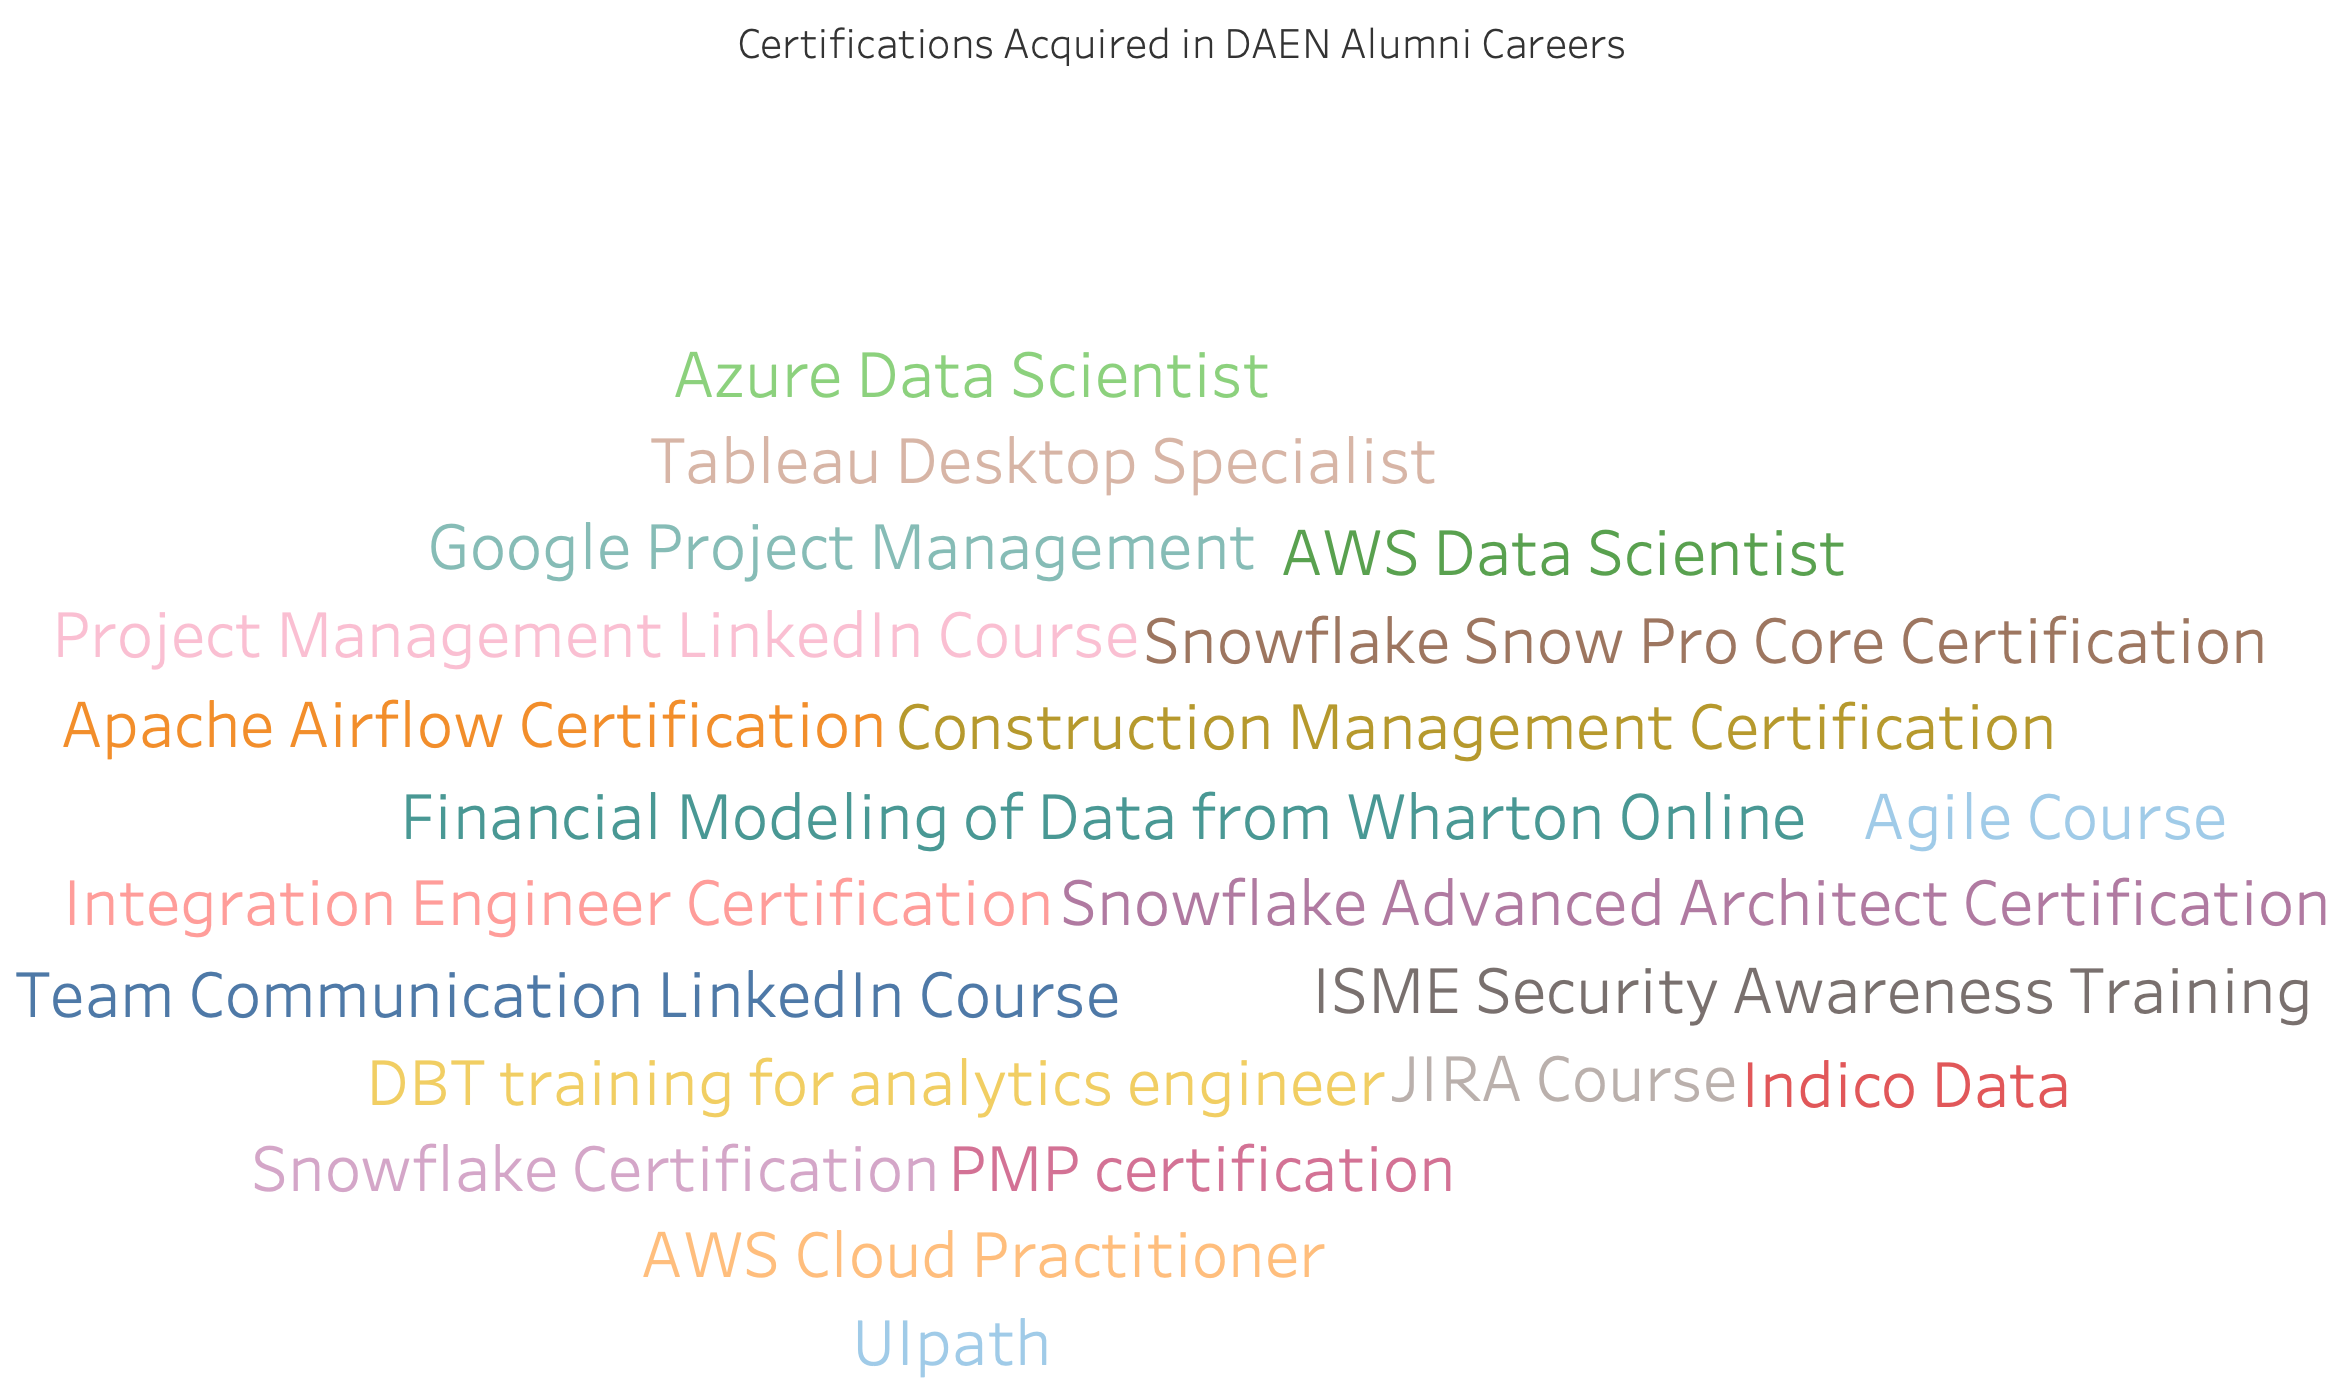
\includegraphics[width=0.9\textwidth]{visualizations/daen-alumni-completed-certs.png}
    \caption{DAEN Alumni Completed Certifications Post-Graduation}
    \label{fig:completed-certifications}
\end{figure}

The alumni reported diverse certifications post-graduation, reflecting individual career paths and employer requirements. 

\newpage

% 6. Findings Section
\section{Findings}
Our comprehensive analysis of alumni interviews revealed several key insights that will help shape the future of the DAEN program:

\noindent\textbf{Program Demographics and Outcomes}
\begin{itemize}
\item Observed concentrated graduate distribution spanning 2019-2023
\item Achieved 100\% MS degree completion rate among all participants
\item Identified average of 2 jobs held by graduates post-graduation
\item Discovered strong representation in data analyst career paths
\end{itemize}
\textbf{Technical Skill Utilization}
\begin{itemize}
\item Documented dominant use of SQL and Python in professional settings
\item Observed high adoption rates of AWS cloud services across roles
\item Tracked increasing importance of Snowflake and Databricks platforms
\item Identified significant focus on visualization tools like Power BI and Tableau
\end{itemize}
\textbf{Program Effectiveness}
\begin{itemize}
\item Measured average program rating of 3.7 out of 5 from alumni
\item Recognized strong satisfaction with database and ML coursework
\item Confirmed high value placed on hands-on project experiences
\item Validated notable impact of DAEN 690 capstone course
\end{itemize}
\textbf{Areas for Enhancement}
\begin{itemize}
\item Identified need for increased cloud computing coverage
\item Recognized demand for more emphasis on practical applications
\item Determined necessity for integration of emerging technologies
\item Discovered need for enhanced focus on industry certification preparation
\end{itemize}

\newpage

\section{Proposed Survey}

\subsection{Survey Overview}
The DAEN program proposes implementing a bi-annual alumni survey to gather ongoing feedback about program effectiveness and industry trends. The survey is designed to be completed in under 5 minutes and focuses on key metrics identified through our initial research.

\subsection{Survey Introduction Message}
\begin{quote}
DAEN Alumni Survey - Spring 2025

This quick survey should take less than 5 minutes to complete. Your responses will help shape the future of the DAEN program at George Mason University. All responses are anonymous and the data will be used solely for program improvement purposes.

Survey Period: February 1st - March 1st, 2025\\
Next Survey Window: September 1st - October 1st, 2025
\end{quote}

\subsection{Proposed Survey Questions}
\begin{enumerate}
\item Which year did you graduate from the DAEN program?
\begin{itemize}
    \item Before 2019
    \item Multiple choice: 2019-2024 (by year)
\end{itemize}

\item What degree type did you receive from the DAEN program?
\begin{itemize}
    \item M.S.
    \item Certificate
\end{itemize}

\item Where do you current work?
\begin{itemize}
    \item US
    \item India
    \item Other (please specify)
\end{itemize}

\item What is your primary job function?
\begin{itemize}
    \item Data Analyst
    \item Data Scientist
    \item Data Engineer
    \item Business Analyst
    \item Machine Learning Engineer
    \item Other (please specify)
\end{itemize}

\item Which industry sector do you currently work in?
\begin{itemize}
    \item Government/Public Sector
    \item Technology
    \item Healthcare
    \item Financial Services
    \item Consulting
    \item Education
    \item Retail
    \item Other (please specify)
\end{itemize}

\item Which programming language do you use most frequently in your current role?
\begin{itemize}
    \item Python
    \item SQL
    \item R
    \item Other (please specify)
\end{itemize}

\item What cloud platform do you primarily use?
\begin{itemize}
    \item AWS
    \item Azure
    \item Google Cloud
    \item Salesforce
    \item None
    \item Other (please specify)
\end{itemize}

\item Which data visualization tool do you use most often?
\begin{itemize}
    \item Tableau
    \item Power BI
    \item Looker
    \item Python Libraries (matplotlib, seaborn, etc.)
    \item Other (please specify)
\end{itemize}

\item Rate your overall satisfaction with how the DAEN program prepared you for your career:
\begin{itemize}
    \item 5 (Extremely satisfied)
    \item 4 (Very satisfied)
    \item 3 (Satisfied)
    \item 2 (Somewhat satisfied)
    \item 1 (Not satisfied)
\end{itemize}

\item Which technical skills from your DAEN education do you use most frequently? (Select top 3)
\begin{itemize}
    \item Database Management
    \item Machine Learning
    \item Statistical Analysis
    \item Data Visualization
    \item Big Data Processing
    \item Cloud Computing
    \item Programming
    \item Data Modeling
    \item Operations Research
    \item Other (please specify)
\end{itemize}

\item Have you completed any professional certifications since graduation?
\begin{itemize}
    \item Yes (please specify in text box)
    \item No
    \item Planning to in next 3 months
\end{itemize}

\item If you have completed any professional certifications since graduation, please specify the certification name(s). (Short text response)

\item What emerging technologies or tools would you recommend adding to the DAEN curriculum? (Short text response)

\item Would you be willing to be contacted for a follow-up interview?
\begin{itemize}
    \item Yes
    \item No
\end{itemize}

\item If you are willing to be contacted for a follow-up interview, please provide your email address. (Short text response)
\end{enumerate}

\subsection{Survey Implementation Schedule}
\begin{itemize}
    \item First Survey Launch: February 1st - March 1st, 2025
    \item Follow-up Survey: September 1st - October 1st, 2025
    \item Annual Schedule: February and September
\end{itemize}

\subsection{Survey Distribution Strategy}
\begin{itemize}
    \item Primary distribution through DAEN alumni email list
    \item Secondary distribution through LinkedIn DAEN alumni group
    \item Reminder emails: Day 5, Day 10, Day 15, Day 20, Day 25
    \item Target response rate: 40\% of reachable alumni
\end{itemize}

\newpage

\section{Next Steps}
Building on our research findings, we have identified several critical initiatives to enhance the DAEN program's effectiveness:

\noindent\textbf{Program Development}
\begin{itemize}
\item Develop automated data pipelines for processing alumni feedback and program metrics
\item Implement secure database systems for managing confidential alumni information
\item Establish comprehensive quality control processes for data management
\end{itemize}
\textbf{Survey Operations}
\begin{itemize}
\item Design standardized survey framework for consistent bi-annual data collection
\item Manage systematic response collection through multiple communication channels
\item Analyze survey results using advanced visualization and reporting toolseffectiveness
\end{itemize}
\textbf{Curriculum Enhancement}
\begin{itemize}
\item Integrate advanced cloud technologies into existing course modules
\item Develop industry-aligned certification preparation programs
\item Update technical curriculum with emerging industry tools and practices
\end{itemize}
\textbf{Alumni Engagement}
\begin{itemize}
\item Launch structured mentorship program connecting students with industry professionals
\item Organize regular professional networking events and technical workshops
\item Create comprehensive online resource center for alumni development
\end{itemize}

\newpage

\section{Lessons Learned}
Our research process yielded valuable insights that will inform future program assessment efforts:


\noindent\textbf{Research Methodology}
\begin{itemize}
\item Recognized importance of early alumni engagement post-graduation
\item Developed standardized questions for actionable feedback
\item Implemented multiple participation methods for broader reach
\item Maintained consistent data formats for efficient processing
\end{itemize}
\textbf{Data Collection}
\begin{itemize}
\item Leveraged professional networks for efficient alumni identification
\item Standardized recording formats for streamlined processing
\item Implemented privacy measures for candid feedback collection
\item Conducted persistent follow-up for sustained engagement
\end{itemize}
\textbf{Process Improvement}
\begin{itemize}
\item Developed automated workflows for accelerated analysis
\item Standardized classification systems for meaningful insights
\item Maintained comprehensive documentation for future reference
\item Incorporated stakeholder input for iterative refinement
\end{itemize}

\newpage

% Appendices
\begin{appendices}
\section{Background}
This research, conducted through DAEN 698: Research Project, represents a significant departmental initiative led by DAEN student and DAEN program director. As the first systematic effort to collect and analyze alumni feedback, this study establishes a foundation for ongoing program assessment and enhancement. The insights gained from this pioneering research will stimulate further discussions and drive continued investment in understanding and improving program effectiveness.

\section{References}
\begin{thebibliography}{9}
\bibitem{gmu} George Mason University. (2024). Data Analytics Engineering, MS. Retrieved from https://catalog.gmu.edu/colleges-schools/engineering-computing/engineering/data-analytics-engineering-ms/
\bibitem{bergelson} Bergelson, I., Tracy, C., \& Takacs, E. (2022). Best Practices for Reducing Bias in the Interview Process. Current Urology Reports, 23(11), 319-325.
\bibitem{nikiforova} Nikiforova, A. (2020). Definition and Evaluation of Data Quality: User-Oriented Data Object-Driven Approach to Data Quality Assessment. Baltic Journal of Modern Computing, 8(3), 391-432.
\end{thebibliography}

\section{Research Biases and Data Quality Considerations}
In conducting this alumni interview research, we identified several key sources of potential bias and inaccuracy that could impact our findings. Despite implementing systematic controls, these factors should be considered when interpreting the results:
\begin{itemize}
\item \textbf{Selection Bias}
\begin{itemize}
\item Sample limited to LinkedIn-active alumni from 2019-2023
\item Response rate of 14 out of 50 contacted alumni
\item Potential over-representation of successful graduates
\end{itemize}
\item \textbf{Data Accuracy}
\begin{itemize}
\item Memory recall variations depending on graduation year
\item Standardization requirements for technical terminology
\end{itemize}
\end{itemize}
While these limitations exist, our methodological controls and transparent reporting help maintain the integrity of the findings while acknowledging areas for potential improvement in future research.

\end{appendices}

\end{document}